\documentclass[12pt]{article}

\usepackage[top=0.75in,bottom=0.75in,left=0.75in,right=0.75in]{geometry}
\usepackage{amsmath,amssymb,multirow,graphicx,natbib}
\usepackage{setspace}

% Comments for making sure we touch all the bases for a good paper
\newif\ifcommentsw
\commentswtrue
\newcommand{\comment}[1]{\ifcommentsw  $\blacktriangleright$\ \textbf{#1}\ $\blacktriangleleft$ \fi}
%\commentswfalse   % remove the % to remove informational comments


% Notes on the paper for communicating with coauthors
\newif\ifnotesw
\noteswtrue
\newcommand{\notes}[1]{\ifnotesw  $\bullet$\ \textit{ \textbf{#1}}\ $\bullet$ \fi}
%\noteswfalse   % remove the % to remove notes to coauthors

\parskip=5pt
\parindent=0pt

\newcommand{\br}{\mathbf{r}}
\newcommand{\sgn}{\operatorname{sgn}}
\def\cq{{\emph{Culex quinquefasciatus}}}
%\newcommand{\mycaption}[1]{\caption{{\footnotesize \textsc{#1}}}}
%\usepackage[font={small,singlespacing}]{caption}
\usepackage[font={small}]{caption}
\newcommand{\mycaption}[1]{\caption{#1}}
\linespread{1.1}

\title{A hybrid model of mosquito-host encounter rates}
\author{
\textbf{Ricardo Cortez}\\
   \small{Mathematics Department}\\
   \small{Tulane University}\\ \and
\textbf{Bree Cummins}\\
   \small{Mathematics Department}\\
   \small{Tulane University}\\ \and
\textbf{Ivo M. Foppa}\\
   \small{Department of Epidemiology}\\
   \small{Tulane University}\\ \and
   \textbf{James M. Hyman}\\
   \small{Mathematics Department}\\
   \small{Tulane University}\\ \and
\textbf{Justin Walbeck}\\
   \small{Mathematics Department}\\
   \small{Tulane University}\\
}


\begin{document}
	
	\tableofcontents
	
	\maketitle

\abstract{
%
%\comment{\it  {\bf Start with the principal result of the paper}}
%
We develop and analyze  a hybrid mathematical model to describe the effect of spatial
heterogeneity on the encounter rate between mosquito vectors and bird hosts.
%
%\comment{\it  {\bf state the problem being addressed and why it is important}}
%
The mosquito host-seeking behavior and heterogeneity in the distribution of hosts are important factors
in predicting the transmission dynamics of mosquito-borne infections  such as the spread of the West Nile virus.
Ignoring heterogeneity in transmission models can result in misleading insights into the  transmission dynamics.
%
%\comment{\it  {\bf what has been done and the bottleneck that has kept the problem from being solved}}
%
%
% \comment{\it  {\bf The objective of this research and how it will advances the solution of the problem}}
%
We present a spatial model that includes odor plumes generated by hosts distributed in space, wind velocity,
and mosquito behavior based on perceived values of wind and odor plume concentration.
The latter is modeled as a continuum spreading by
diffusion and carried by the wind, while the mosquitoes and hosts are modeled as discrete points with
behavioral rules that depend on the local conditions.  The wind is composed of a functional component plus
a stochastic component to represent small scale variations.
%Mosquitoes use a variety of host seeking strategies in guiding them to a blood meal.  When odor plumes and not present, the mosquitoes engage in ranging flight behavior, influenced by the wind velocity.  When they pick up the scent of a host, then their flight is influenced by both the wind velocity and odor cues.
%
%\comment{\it  {\bf State the principal results}}
%
%Our model includes behavioral rules for the
%flight of discrete host-seeking mosquitoes, a continuum model for the spreading odor plume
%generated by resting hosts, and stochastic non-uniform wind conditions.
We model several proposed strategies for odor-tracking in the absence of wind to locate a host and quantify their relative effectiveness.
A sensitivity analysis to the full wind-driven model shows robustness with respect to changes in parameter values.
The results are most sensitive to the maximum mosquito flying speed, the amount of time mosquitoes spend moving
in one direction when they fly in a crosswind pattern, and the distance at which vectors turn to visual cues
once they spot a host.
We investigate the effect of mosquito behavior in response to wind direction and the effect of host arrangement on the number of mosquito-host contacts. The greatest number of contacts occurs using a strategy of flying across the wind until the odor plume is intercepted. More contacts also occur when hosts are distributed less densely in the center of the computational domain, resulting in a wider odor plume.
%
%\comment{\it  {\bf How these results advance the understanding of the problem}}
%
Overall, our hybrid model indicates that small-scale heterogeneity in host distribution and mosquito behavior leads to noticeable changes in contact rate.
}
\par
\comment{I shortened the abstract a little:
We develop and analyze  a hybrid mathematical model to describe the effect of spatial
heterogeneity on the encounter rate between mosquito vectors and bird hosts.
The mosquito host-seeking behavior and heterogeneity in the distribution of hosts are important factors
in predicting the transmission dynamics of mosquito-borne infections  such as the spread of the West Nile virus.
Ignoring heterogeneity in transmission models can result in misleading insights into the  transmission dynamics.
Our model includes odor plumes generated by spatially distributed hosts, wind velocity,
and mosquito behavior based wind velocity and direction and odor plume concentration.
We model several proposed strategies for odor-tracking in the absence of wind to locate a host and quantify their relative effectiveness.
A sensitivity analysis indicates that maximum mosquito flying speed, the amount of time mosquitoes spend moving
in one direction when they fly in a crosswind pattern, and the distance at which vectors turn to visual cues
once they spot a host are most influential on the simulation results.
Our simulations suggest that the host finding is optimized by a strategy of flying across the wind until the odor plume is intercepted. Finding hosts is facilitated by less densely distributed hosts because resulting odor plume is wider.
Overall, our hybrid model indicates that small-scale heterogeneity in host distribution and mosquito behavior leads to noticeable changes in contact rate.
}


\textbf{Keywords} mosquito $\cdot$ mathematical model $\cdot$ West Nile virus  $\cdot$ odor plume $\cdot$ chemotaxis $\cdot$ agent-based model
	
%%%%%%%%%%%%%%%%%%%
\section{Introduction}
%%%%%%%%%%%%%%%%%%%
%\comment{\it  {\bf Make it clear to the reader what the main idea of the paper is after the first 3-5 paragraphs of the introduction and give a clear picture of what is to come in the paper.   }}

The transmission of infectious agents is heterogeneous in the sense that the risk for infection and infectiousness are unevenly distributed over the population~\cite{Woolhouse1997}. This heterogeneity is an important factor in predicting the spread of an infection; ignoring it may result in misleading inference about transmission dynamics by underestimating the probability that an infectious agent will persist ~\cite{Hasibeder1988}.  One source of heterogeneity in mosquito-borne disease transmission is the nonuniform distribution of mosquito bites over hosts~\cite{Dye1986} (per-capita biting rates). The number of mosquitoes that bite a host depends, among other things, on the number that find it.
Host finding by mosquitoes is largely driven by olfactory cues that are given off by individual
hosts~\cite{Lehane1991}.
The spatial arrangement of hosts is likely to affect the spatial distribution of the odor plume and thus the mosquitoes' ability to locate and feed on them. For example, it may be easier for a mosquito to find a large roost of birds than to find an single bird.  Unless the probability of finding a host is exactly proportional to the density of hosts, unevenly distributed contact rates on individual hosts and thus heterogeneous disease transmission will result.  Understanding the dynamics of odor-driven mosquito-host interaction is fundamental to a detailed mechanistic understanding of mosquito-borne transmission.

%This is an important observation for the American crow (\textit{Corvus brachyrhynchos}) and other species of birds that are particularly vulnerable to WNV infection and tend to congregate in large roosts.  An immediate question is {\em How does the roosting behavior of birds and catastrophic changes in roost structure affect the transmission dynamics of this mosquito-borne virus?} Answering this question motivates the work presented here. It requires a detailed understanding of how the spatial arrangement of hosts will affect the distribution of mosquito bites on these hosts.
%

We develop and analyze a mathematical model
to simulate  both the odor plume in the presence of wind and the host-seeking behavior of mosquitoes in response to that odor plume. Mosquitoes are modeled as discrete {\em agents} that fly in a continuous ``odorscape'' in search of  discrete hosts (birds).
The wind is composed of a function for the large scale component plus
a stochastic component to represent small scale variations.
The flight direction and speed of individual mosquitoes is influenced by both the wind and odors
emitted by the hosts.


The model is flexible enough that wind patterns, spatial distribution of hosts, and behavioral rules of the mosquitoes can be changed within the same framework.  This allows us to compare the effectiveness of different mosquito flight strategies in finding a host.  We also evaluate the difference between host-seeking models based on the local concentration of the odor plume and/or the gradient of the odor plume. We
quantify the sensitivity these models to assumptions about model parameters.
The end result is a robust model that can be used under a wide range of conditions and that serves as a virtual laboratory for testing different hypothesis for how mosquitoes use odor plumes to locate potential hosts.
This framework could serve as a virtual laboratory for exploring the effects of small-scale spatial heterogeneity on the transmission of vector-borne disease.
\comment{What is the consensus on this last sentence? Is it a reasonable claim? BC  I like it. MH}

%We will first review the host-seeking behavior of mosquitoes, then ...




 %We find that the there are a broad range of effective host-seeking strategies that are insensitive out detailed assumptions of the parameter values.

%We will use mathematical modeling to address the effect of host aggregation on a small-scale spatial on the per-capitabiting rate.   Specifically, we present a model for the simulation of host-seeking behavior of mosquitoes that applies to the transmission of West Nile Virus or other mosquito-borne diseases.  The model accounts for host-seeking behavior in both ranging flight, influenced by wind velocity, and homing flight, guided by both wind velocity and odor cues.  There is little experimental data for the parameters in a host-seeking mosquito model.  We use sensitivity analysis to quantify the uncertainty in our predictions as a function of changes in our assumptions.   The sensitive analysis shows that the ability of mosquitoes to find a host is relatively insensitive to our model assumptions. We find that under some conditions, these different approaches are both effective and do not show statistically significant differences in a mosquito's ability to locate a host.

%\comment{\it  {\bf After the introduction, the reader should understand the importance of this problem and what contribution the authors made to solving a problem. }}

%%%%%%%%%%%%%%%%%%%%%
\section{Mosquito host-seeking behavior}\label{sec:mosqbehav}
%%%%%%%%%%%%%%%%%%%%%%
The diurnal cycle triggers host-seeking behavior in mated female mosquitoes. \comment{citation} Typically this behavior begins when the mosquitoes are far from the hosts and ends after a successful bite.  We model mosquito host-seeking behavior between tens of meters and tens of centimeters from a host. On this scale, it is useful to classify the behavior in terms of two functional regimes that we will call  {\em homing flight} (flight influenced by the presence of an odor cue) and {\em ranging flight} (flight without an odor cue).

%%%%%%%%%%%%%%%%%%%%%%
\subsection{Ranging flight}
%%%%%%%%%%%%%%%%%%%%%%
In the absence of odor cues, mosquitoes use ranging flight, influenced by wind currents, to locate odor plumes.  Unlike homing flight (see below), there is no consensus about mosquito ranging flight behavior. If wind is absent, orientation may be determined by large visual features in the
environment~\cite{Bidlingmayer1994} or may be characterized as an unbiased random walk. If wind is present, then mosquitoes may deliberately choose to fly upwind, downwind, or crosswind in search of a host.  Each of these three behaviors has been described as plausible based on either experimental or theoretical work.
Mosquitoes typically fly upwind in wind tunnels even when there is no odor present~\cite{Gibson1999}.
A set of field experiments reported in~\cite{Gillies1974} provided evidence for downwind flights in host-seeking
 \emph{Mansonia} mosquitoes.
In~\cite{Dusenbery1989} it is argued that crosswind searching is optimal in some sense when the odor plumes are long and thin.  If the variability of the wind direction is greater than 30 degrees, then there is evidence that either upwind or downwind searching becomes optimal~\cite{Sabelis1984}.  We will compare the effectiveness of these three ranging flight behaviors in locating a host in our model equaitons.

%%%%%%%%%%%%%%%%%%%%%%
\subsection{Homing flight}
%%%%%%%%%%%%%%%%%%%%%%
When a mosquito detects an odor plume from a host, it uses the odor plume and the wind to guide its homing flight to locate the host.
Odor cues are complex olfactory signals released from a host's skin and breath. Many compounds are known to excite the chemoreceptors of mosquitoes.
%
CO$_2$, for example, is a important component in the odor plume that activates and helps maintain homing flight~\cite{Bowen1991,Gibson1999,Gillies1980}. The importance of lactic acid, and various
aldehydes for the location of hosts by mosquitoes has also been demonstrated~\cite{Bowen1991,Syed2009}.
There is typically a CO$_2$ activation threshold for the mosquitoes as well as a minimum concentration change that mosquitoes can sense.








Both the odor plume concentration and its {\em structure} are important to the  host--seeking behavior of mosquitoes. Laboratory wind tunnel experiments indicate that
sustained flight only occurs in the presence of an intermittent CO$_2$ signal and not in uniform
concentrations~\cite{Gillies1980}.  Other wind tunnel experiments suggested that broad,
well-mixed CO$_2$ plumes may inhibit upwind flight while turbulent plumes of the same concentration induce
upwind flight~\cite{Dekker2005,Dekker2001}.

Since air is the medium where the dynamics of the odor plume take place, the plume concentration is both carried by the wind (convection) and diffuses in the air in the same way that a puff of smoke dissipates in time.
Uniform, laminar wind tends to extend host odor into a long, thin plume with sharp transverse gradients and shallow longitudinal gradients. If the wind is turbulent, the plume has been hypothesized to be highly intermittent, while still retaining relatively shallow average longitudinal gradients compared to the transverse
gradients~\cite{Vickers2000}.


Mosquitoes exhibit different behavior in windy and windless conditions. In the absence of wind within the odor plume, mosquitoes must rely solely on odor cues~\cite{Vickers2000} or on large features in the visual environment~\cite{Bidlingmayer1994}. Mosquitoes may sample the odor over time to estimate the gradient, as is conjectured for tsetse flies~\cite{Carde1996}.
%
Laboratory and field wind tunnel experiments suggest that under windy conditions within the odor plume, the mosquitoes travel upwind to locate the source~\cite{Cooperband2006, Dekker2005,Dekker2001}. Mosquitoes appear to infer wind direction from the optical flow of ground features relative to their position~\cite{Carde1996}.
It is known that many organisms have characteristic turns in their upwind flight path (e.g. moths~\cite{Carde1996,Vickers2000}), but mosquitoes and tsetse flies exhibit highly irregular upwind flight~\cite{Davis1996}.




%%%%%%%%%%%%%%%%%%%%%%
\section{Model Formulation}
%%%%%%%%%%%%%%%%%%%%%%
% \comment{\it{\bf Describe how the model was developed to answer the research question.
% Give full details of the chosen methodology so that an interested reader could repeat it.
%Follow a logical order, usually from simple to more complex, or chronological.
%A graphic image, which visualizes the model, can be an effective and important attention-grabber. Don't hesitate to use extended figure captions that fully describe the figure (including defining the the axes of all graphs).  Be sure to point out explicitly what you want to reader to see in each figure.  Don't assume that the reader will see what you think is obvious.  Use an adequate font size in the figure and be sure that the text on your figures does not require a magnifying glass to read.
%}}


We envision night--active mosquitoes such as \textsl{Culex quinquefasciatus} feeding on roosting birds.   We construct a modeling framework that can accommodate different ranging and host-seeking mosquito behaviors, wind velocities, host locations, and other physical and biological scenarios.  The model is two-dimensional so that all of the dynamics are assumed to take place at a fixed distance from the ground.
Below, we describe in detail the various components of the model.










%%%%%%%%%%%%%%%%%%%%%%	
\subsection{Odor plumes}
%%%%%%%%%%%%%%%%%%%%%%
Hosts emit CO$_2$, or another gaseous compound, which is carried (convected) by wind
and diffuses in the air.  The CO$_2$ distribution over time is modeled by a convection-diffusion partial differential equation.  If the convection velocity of the wind is given by
a velocity vector ${\vec V}(x,y,t)$, the concentration $C(x,y,t)$ of CO$_2$ is described by the  equation
\begin{equation}\label{eq:conv-diff}
\frac{\partial C}{\partial t} + \nabla\cdot ( {\vec V} C ) = D\nabla^2 C + C_s(x,y),
\end{equation}
\[
\mbox{with\ \ \  } \vec{V}(x,y,t) = \vec{U}(x,y,t) + \vec{U_r}(x,y,t)
\]
where $t$ is time, and $(x,y)$ are spatial coordinates.  The constant diffusion coefficient $D$ can be adjusted to reflect the speed at which the particular substance of interest diffuses in air.
The transport velocity $\vec{V}$ consists of two components: $\vec{U}$ is used to introduced drifts or
relatively large features produced by the air;
$\vec{U}_r$ is a random velocity vector with mean zero
introduced to approximate the effect of small-scale wind variations in the domain.  The last term
in Eq.~(\ref{eq:conv-diff}) represents the source of CO$_2$ concentration at the host locations.
In this work we consider hosts that release a fixed amount of CO$_2$ per host per
unit time. However, this is not a limitation of the model and can be changed.
%In our model, we will consider this term to be
%\comment{\textsl{I would put the following expression on a separate line IF}}
%$C_s(x,y) = J_0 \int\!\!\!\int \delta(x-x_h-z_1,y-y_h-z_2) dz_1 dz_2$ where $J_0$ is a constant
%concentration emission per unit time and the delta function reflects the fact that the CO$_2$
%occurs only at the host locations $(x_h,y_h)$.
		
We simulate the evolution of the CO$_2$ concentration on two-dimensional rectangular domain $[0,L] \times [0,L]$ with uniform grid spacing $h = L/N$.  We use second-order centered differences to approximate the Laplacian and  a first-order conservative upwind finite difference method for the convection terms. We assume that the normal components of the concentration gradient are zero at the boundary (Neumann conditions) and the large scale air motion is incompressible $\nabla\cdot \vec{U} = 0$.  We integrated the equations with a forward Euler method and verified that the solutions have converged in the $L_2$ norm.

%%%%%%%%%%%%%%%%%%%
\subsection{Mosquito Behavior}
%%%%%%%%%%%%%%%%%%%
We model and track mosquitoes and hosts as discrete individuals, or
agents. Motivated by the
encounter rate between birds and \textsl{Cx. quinquefasciatus}
mosquitoes, which is a nocturnal species, the principal
opportunities for host-mosquito interaction are during roosting
periods in which the birds are relatively stationary. For this
reason, the agents representing bird hosts do not move from
their initial positions; however, random walks or other type of
motion could be easily introduced. Mosquitoes move by making short flight segments with
direction and speed selected from a behavioral rule set with a stochastic component.
% The mosquito locations are not restricted to the CO$_2$ grid.
%
A population of $N_v$ mosquitoes are released at the same time with independent entrance locations into the domain.
Initial populations of $N_h$ hosts (e.g. birds) are placed in subregions of the domain.

Our model accounts for two distinct mosquito behavioral
regimes: ranging flight that occurs before a CO$_2$ signal is
detected, and homing flight that occurs in the presence of
sufficient CO$_2$.    Each mosquito flight segment over a time segment
interval of length $\Delta T$ is defined by direction and
speed. (Note that the $\Delta T$ for a mosquito flight segment is
independent of the time step used for numerically solving the
equation (\ref{eq:conv-diff}).)  For each mosquito we first compute a {\em target}
direction $\theta$ and a corresponding angle interval
$[\theta-\alpha, \theta+\alpha]$ based on the wind direction
and CO$_2$ concentration (see below).  A flight segment is then taken in
the direction chosen from a uniform distribution in the
interval. This can result in the mosquito losing the  CO$_2$
signal.

The speed of the segment is chosen between a maximum and a minimum
imposed speed and is found through a deterministic function of
concentration and wind speed. A detailed description is given
below. Our model assumptions about mosquito behavior include:
\begin{itemize}
\item
Below a CO$_2$ threshold $C_0$, the mosquitoes navigate only using wind direction and move according to a predetermined upwind, downwind, or crosswind pattern.
\item For concentrations above the threshold, the
    mosquitoes respond by moving both upwind and
   up the gradient of CO$_2$. There are saturation levels
    $C_{sat}$ and $G_{sat}$ above which no further changes
    in concentration or concentration gradient can be
    detected.
\item Large concentrations and large concentration
    gradients strongly bias the mosquito flight direction and lead to narrower angle windows from which a
    mosquito chooses its direction.
\item  Low concentrations and small concentration
    gradients weakly bias the mosquito flight direction and lead to wider angle windows from which a
    mosquito chooses its direction.
\item The mosquito motion is not restricted to the CO$_2$
    grid. Additionally, the mosquitoes may leave and re-enter the
    concentration computational domain.
\item When a mosquito
comes within a predetermined radius
    $r_c$ of a host, the mosquito is removed from the
    simulation and a ``contact" is recorded. In this
    context, a contact means an attempted landing or bite,
    not necessarily successful.
\end{itemize}
	
	
	We now describe the detailed rules for chemotactic mosquito flight up the gradient of the odor plume by either assuming that the mosquito biases its flight by sensing local concentration gradients or by assuming the flight behavior is based only on  local odor concentration levels.

%%%%%%%%%%%%%%%%%%%%%
\subsubsection{Mosquito direction by sensing concentration gradients}
%%%%%%%%%%%%%%%%%%%%%
Consider a model of mosquito directional behavior based on
concentration gradient.  The CO$_2$ gradient $\nabla C$ is computed on the
grid using finite differences and then it is interpolated to
the mosquito location.  The direction $\theta$ of the gradient
is defined as the target direction for the mosquito's next flight
segment. Given that there is inaccuracy in the ability for a
mosquito to determine this direction, we produce a window of
directions from which the mosquito will choose randomly.  The
size of the window varies inversely with the magnitude of the
concentration gradient as follows.

Let $G_{sat}$ be the maximum concentration gradient that can be
sensed and define the normalized gradient at  the mosquito
location by $b = |\nabla C|/G_{sat}$.  Let the threshold
concentration gradient be a proportion of the saturation
gradient $G_0 = b_0\ G_{sat}$ (with $0<b_0<1$) and let $\kappa$
be any number in the range $(-1/b_0,\infty)$.  The window
$[\theta-\alpha,\theta+\alpha]$ (see
Fig.~\ref{MosquitoGradient}) is computed from
\begin{equation} \label{eqn:response}
\alpha = \alpha_{max} - (\alpha_{max}-\alpha_{min}) F(b,b_0;\kappa)
\end{equation}
where $\alpha_{max}$ and $\alpha_{min}$ are predetermined parameters and the transition function is set to
\begin{equation}
F(b, b_0; \kappa) = \left\{ \begin{array}{lr}
   0, & b < b_0 \\
   \dfrac{(1+\kappa b_0)(b-b_0)}{(1+\kappa b_0 b)(1 - b_0)}, & b_0 \leq b \leq 1 \\
   1, & 1 < b
   \end{array}\right. . \label{eqn:functional}
 \end{equation}
This ensures that the interval size $\alpha$ takes on the highest values when the sensory input is lowest. The parameter $\kappa$ controls the concavity of the transition function as shown in Figure~\ref{MosquitoGradient}.
Once the window of possible flight segment directions is found, the mosquito picks a direction given by a
random variable uniformly distributed in the window interval: $\theta_c \in [\theta-\alpha,\theta+\alpha]$.
The maximum angle $\alpha_{max}$ is fixed at $\pi$ to ensure an unbiased random walk far from the source.

%\begin{figure}[htp]
%\begin{tabular}{ccc}
%	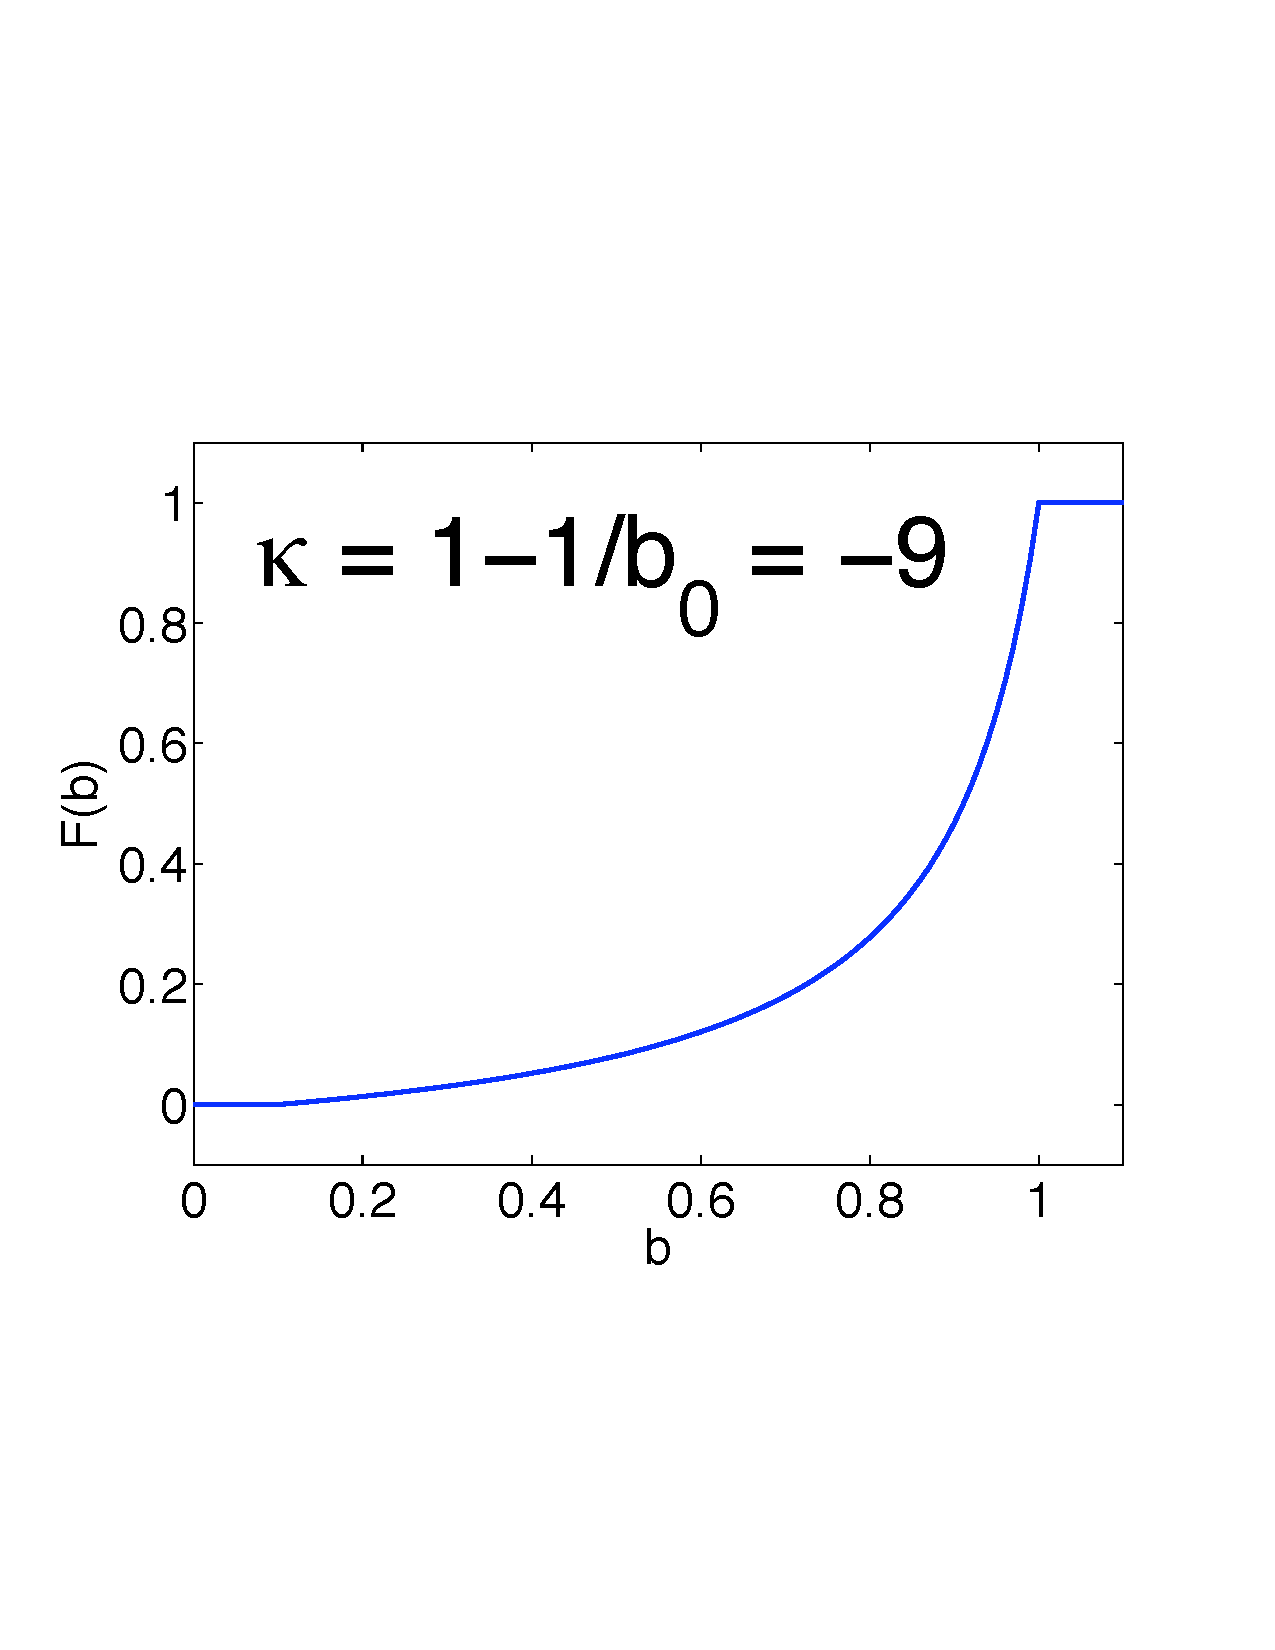
\includegraphics[width=2.25in]{figures/Fconcaveup.pdf} & 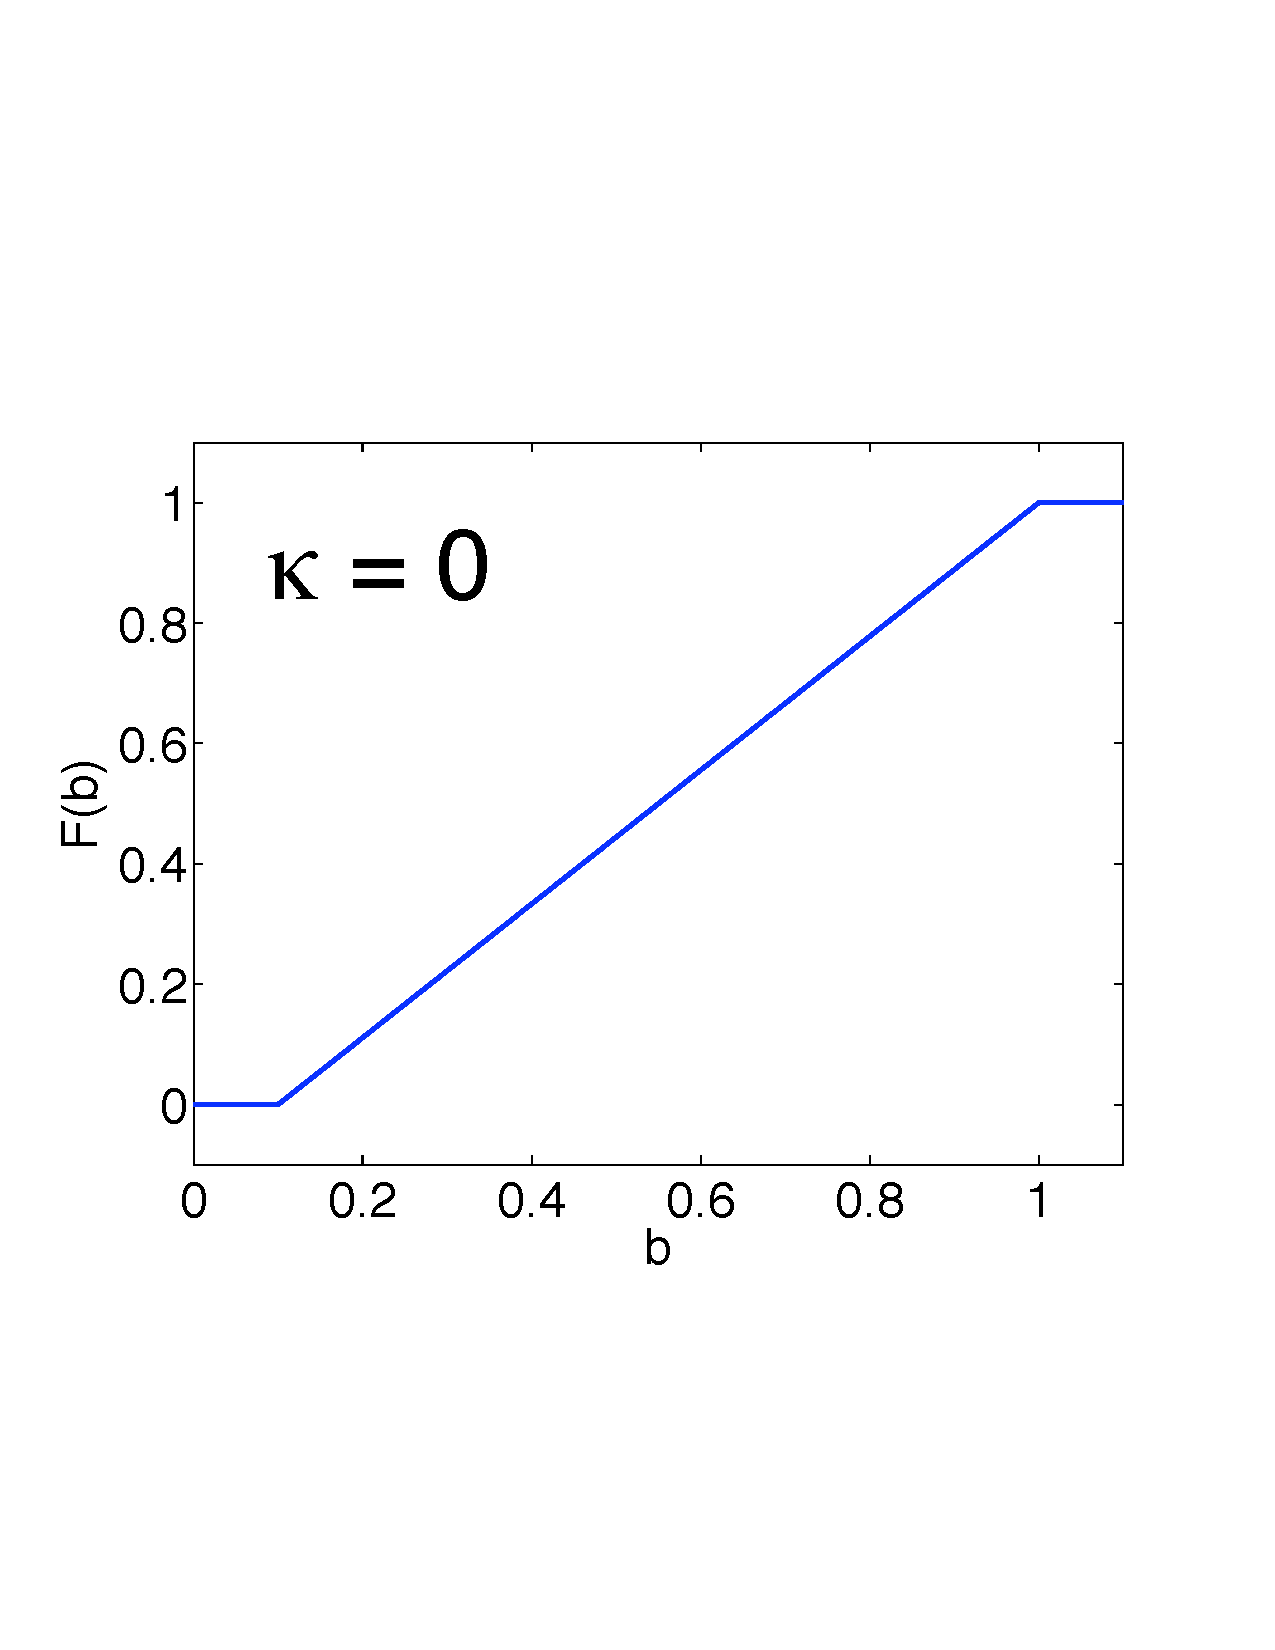
\includegraphics[width=2.25in]{figures/Flinear.pdf} & 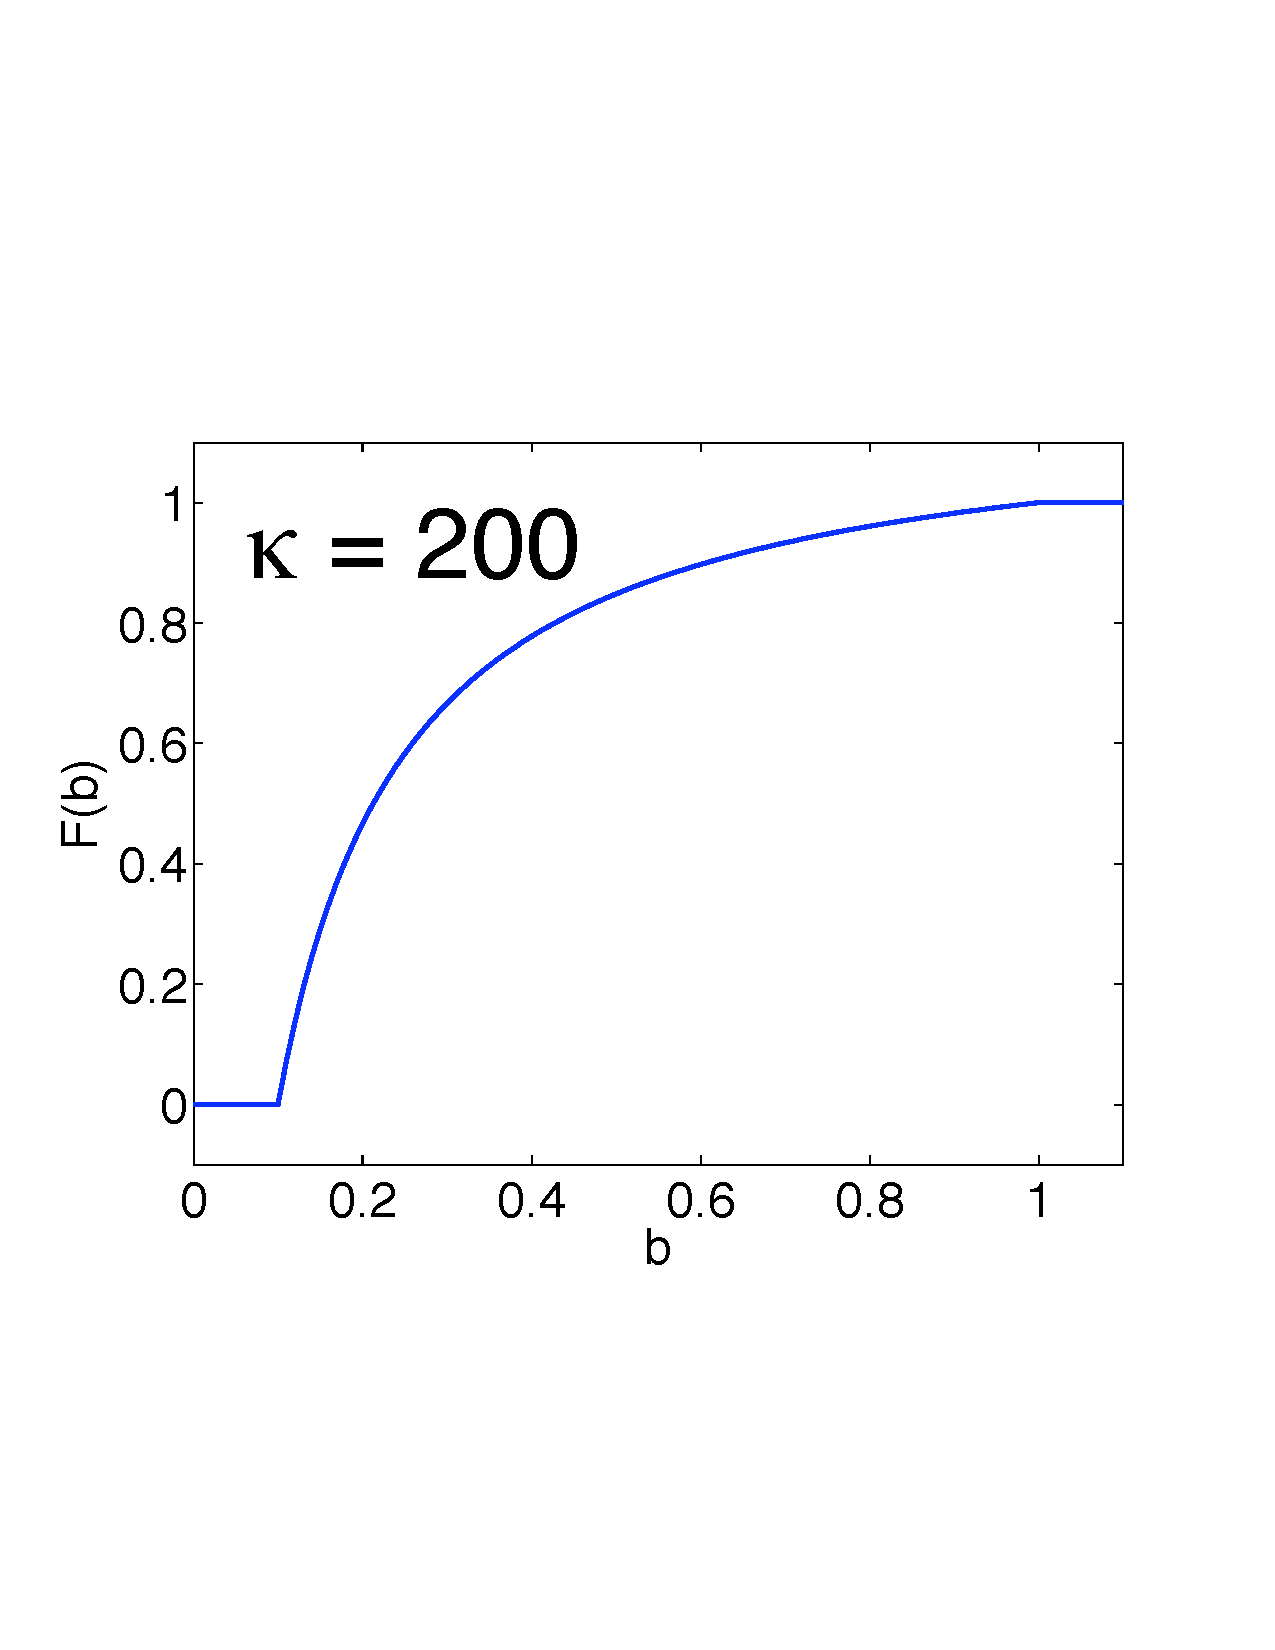
\includegraphics[width=2.25in]{figures/Fconcavedown.pdf}
%\end{tabular}
%\mycaption{
%The shape of the transition function \ref{eqn:functional} as a function of the normalized concentration gradient $b$
%is controlled by the parameter $\kappa$.  When $\kappa < 0 $, $F(b)$ is convex and the mosquito is slow to respond to lower concentration gradients.  When $\kappa >0 $, $F(b)$ is concave and the mosquito is quicker to respond to lower concentration gradients.
%For these figures, $b_0 = 0.1$.
%\comment{These three figures would be better if they were combined to create a single larger figure with three curves for $\alpha$ instead of 3 plots for $F$ and put the figure side-by-side with Figure 2.}
%}
%\label{fig:exampleF}
%\end{figure}

\begin{figure}[hbt]
\centering
 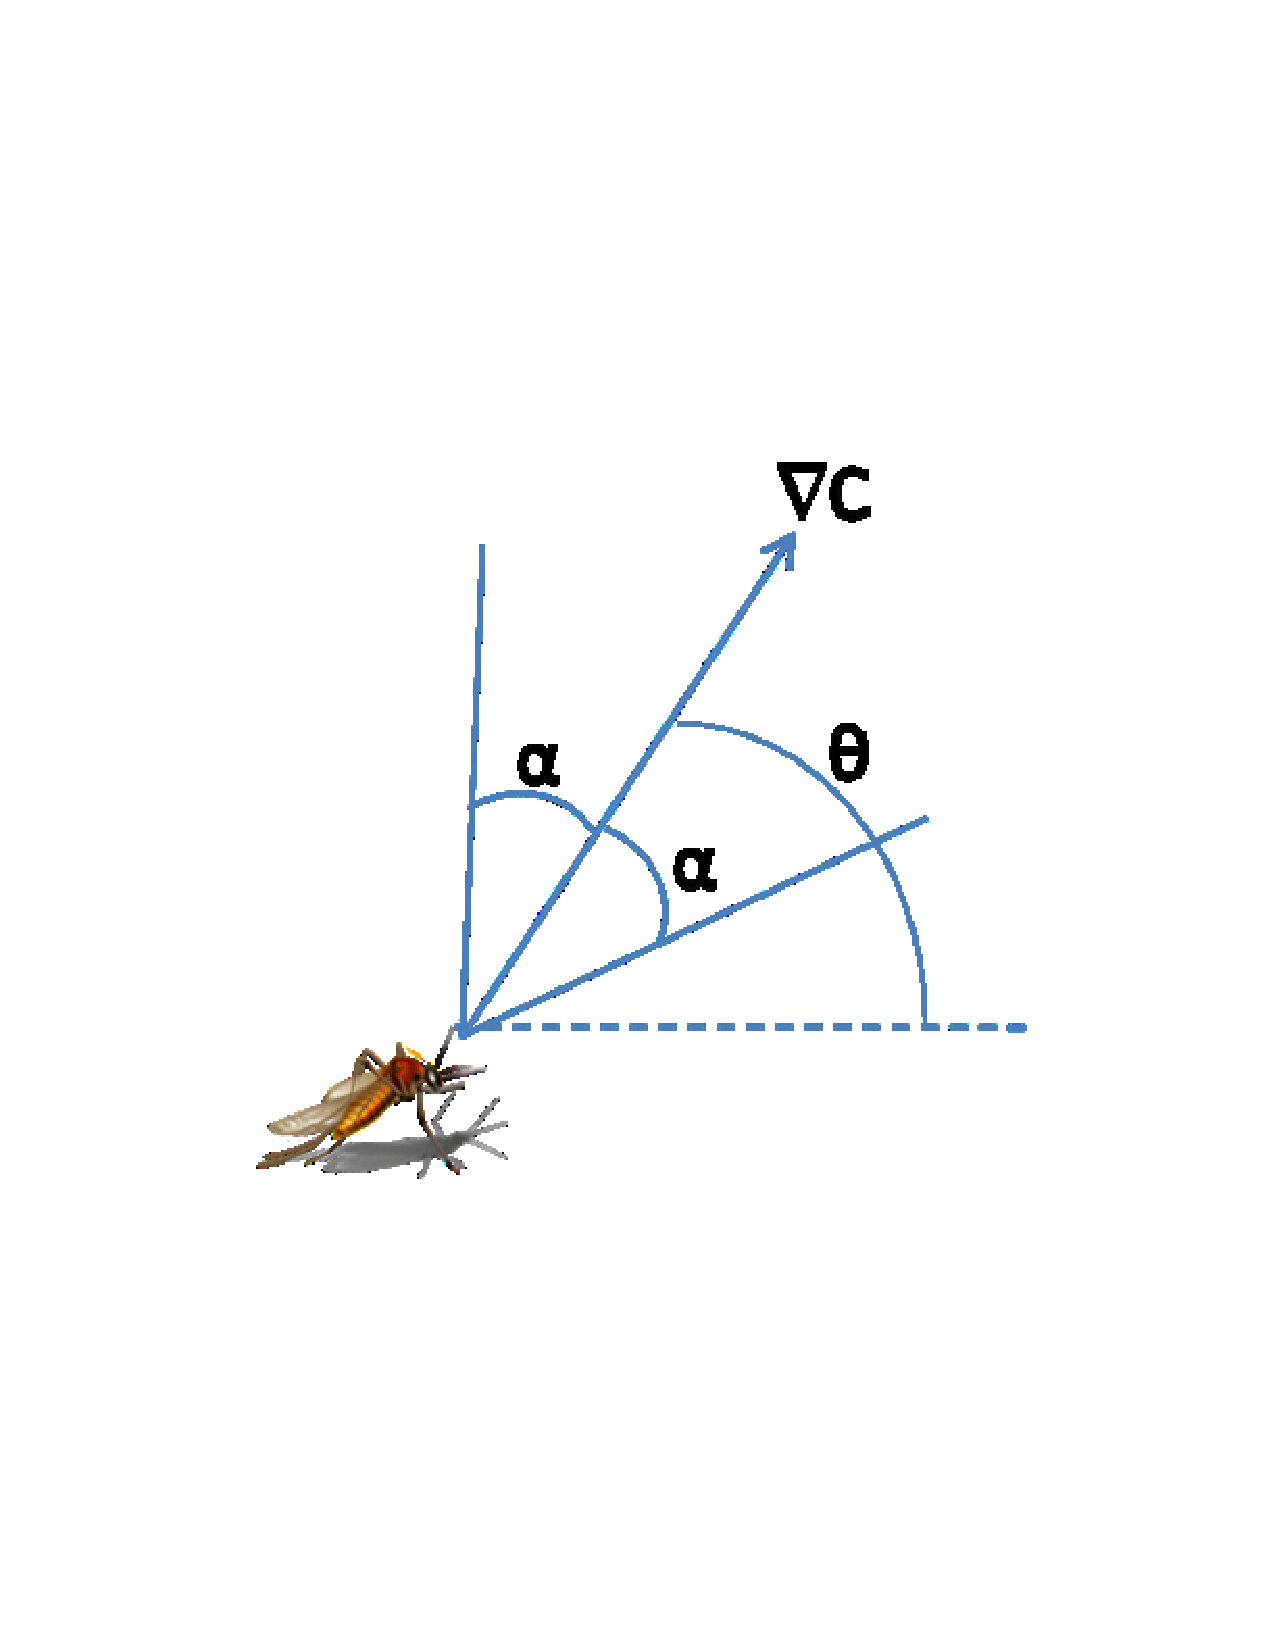
\includegraphics[width=2.5in]{figures/GradientWalkSchematic.pdf}\hskip30pt
 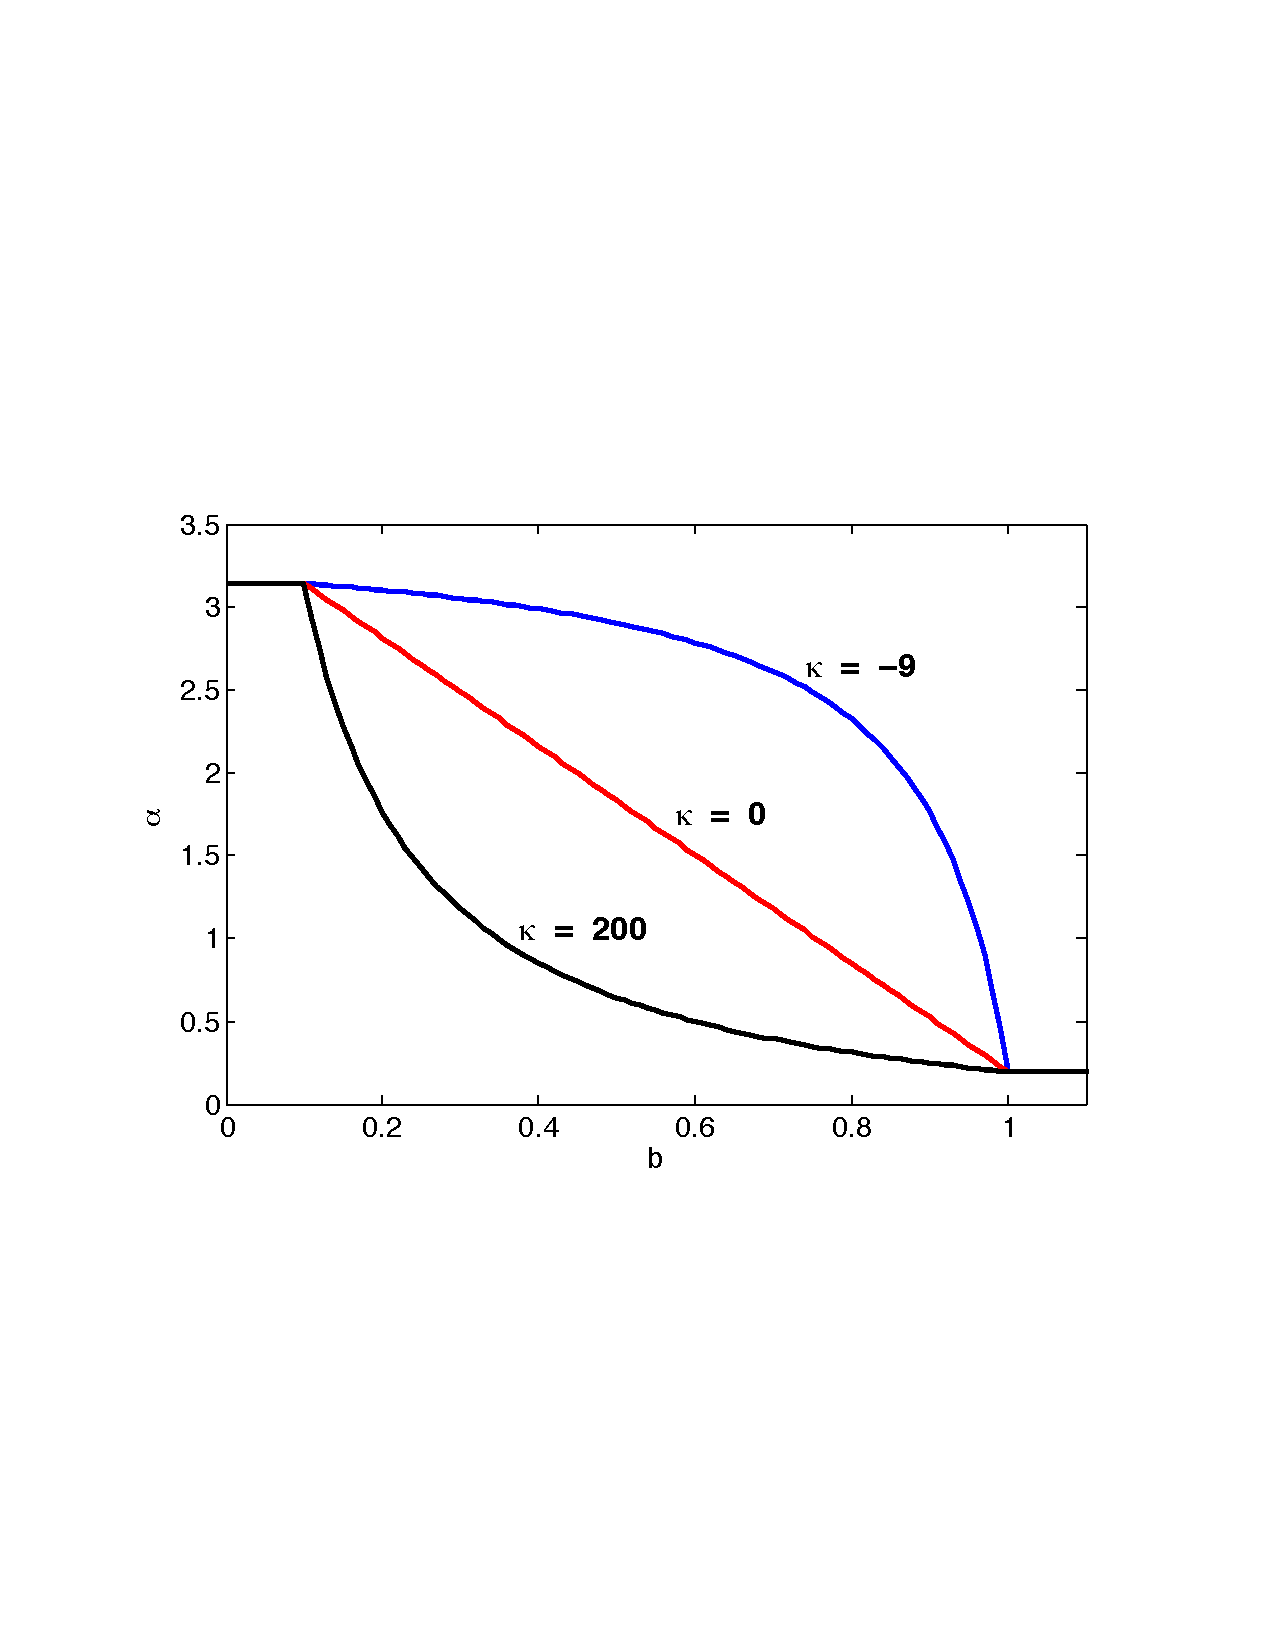
\includegraphics[width=3.1in]{figures/wnvFig1.pdf}
\mycaption{(Left) Schematic of the mosquito host-seeking model based on the concentration gradient direction. At each discrete flight segment, the angle $\theta$ represents the actual direction of the gradient, which the mosquito can only sense to within a precision of $\alpha$.  (Right) Example of the angle $\alpha$ as a function of $b$ as defined in Eq.~(\ref{eqn:response}). When $\kappa < 0 $, $\alpha$ is concave down and the mosquito is slow to respond to higher concentration gradients.  When $\kappa >0 $, $\alpha$ is concave up and the mosquito is quicker to respond to higher concentration gradients. When $\kappa = 0$ the function is linear. In this example, $b_0 = 0.1$, $\alpha_{min} = \pi/16$ and $\alpha_{max} = \pi$.}

\label{MosquitoGradient}
\end{figure}



%%%%%%%%%%%%%%%%%%%%%%%
\subsubsection{Mosquito direction by sensing concentration level}
%%%%%%%%%%%%%%%%%%%%%%%
The mosquito may instead choose a flight segment direction based comparing on the local CO$_2$ concentration with the concentration previously encountered. This is equivalent to monitoring a temporal gradient of the concentration in the direction of its last flight segment.  In this case, the behavioral rules are:
\begin{itemize}
\item
If the current concentration at the mosquito location is larger than the
concentration at the previous segment, the direction used in the previous segment becomes the new target direction
$\theta$.
\item
If the current concentration at the mosquito location is lower than the
concentration at the previous segment, the target direction is set to the reverse of the one used in the previous segment.
\item
A saturation concentration change $\Delta C_{sat}$ is used as the maximum concentration
change that can be sensed.  A threshold concentration change $\Delta C_0 = b_0\ \Delta C_{sat}$
(with $0<b_0<1$) is used as the minimum concentration change that can be sensed.  In this way, concentration changes below this threshold are imperceptible.
\end{itemize}
A window of directions centered around $\theta$ is computed as before except that the gradient
magnitude is replaced by the difference $C(x_n,y_n,t_n)-C(x_{n-1},y_{n-1},t_{n-1})$. Here $(x_n,y_n)$ is the mosquito location at time $t=t_n$. The window of possible flight segment directions is again given by Eq.~(\ref{eqn:response}), but in this case $b = |C(x_n,y_n,t_n)-C(x_{n-1},y_{n-1},t_{n-1})|/\Delta C_{sat}$.
	
%%%%%%%%%%%%%%%%%
\subsubsection{Mosquito direction effect due to wind velocity}
%%%%%%%%%%%%%%%%
The mosquito flight is always affected by the wind velocity when it is present. In our simulations, we interpolate the wind velocity from the grid points to the mosquito locations.
As before, we model the wind sensing capability of the mosquitoes as a precision window around the direction of the wind and we choose a random direction within this precision window.  The randomness of the mosquito response is intended to mimic the average behavior that would occur based on visual cues over many possible ground patterns. We consider wind speeds lower than the typical flight speed for mosquitoes, 1 m/s or less~\cite{Clements1999}, so that the mosquitoes fly at speeds greater than the mean wind speed and upwind flight is possible. 	

In the model, mosquitoes have an assigned flight strategy: downwind, upwind, or crosswind.
Let $\theta_v$ be the direction of the wind $\vec V$ at the mosquito location.  Then the mosquito target direction is $\theta = \theta_v + \psi$, where $\psi=0$ for downwind flight, $\psi=\pi$ for upwind flight, and $\psi \in [-\pi/2, -\pi/4] \cup [\pi/4,\pi/2]$ for varying degrees of crosswind flight.  As before, the direction is chosen randomly from a window
$[\theta-\alpha,\theta+\alpha]$ where $\alpha$ is given by Eq.~(\ref{eqn:response}) with $b = |\vec{V}|/V_{sat}$ and the threshold speed by $V_0 = b_0\ V_{sat}$:
\begin{equation*}
	\theta_w \in [\theta_v + \psi-\alpha,\theta_v + \psi+\alpha]. %\label{eqn:vdirchoice}
\end{equation*}

During crosswind ranging behavior, a mosquito will oscillate
between traveling to the right and left of the wind direction.
The duration of the travel in one direction is a parameter in
the model. We choose this duration to be uniformly selected
from an interval $T_{cwd} = [T_{min},T_{max}]$.
\comment{Bree - can you please elaborate on just what the cross wind behavior is.  I could not reproduce it from what we've described in this paragraph.  Thanks, MH}

%%%%%%%%%%%%%%%%%
\subsubsection{Mosquito flight speed selection}
%%%%%%%%%%%%%%%%
Once the mosquitoes have chosen a flight direction, they must also select a speed for the next flight segment.  We assume that the speed of a mosquito is bounded between a minimum
$S_{min}$ and a maximum $S_{max}$.  Unlike the random choice of direction, the speed of the
 mosquito is defined by a deterministic formula
\begin{equation}\label{eqn:speed}
	s = S_{max} - (S_{max} -  S_{min})F(b, b_0; \kappa).
\end{equation}
where the variable $b$ represents the normalized CO$_2$ concentration $C/C_{sat}$ at the mosquito location.  Because of the nature of the function $F(b, b_0; \kappa)$, if the concentration is below the threshold $C_0$, then the mosquito speed becomes $S_{max}$.  Similarly, if the concentration sensed by the mosquito is above $C_{sat}$, then the segment speed is $S_{min}$.  This allows mosquitoes to remain near areas of high concentration.  The mosquito speed may be set to a constant by simply choosing $S_{min} = S_{max}$.

%%%%%%%%%%%%%%%%%%%%%%%%%
\subsubsection{Summary of mosquito behavior model}
%%%%%%%%%%%%%%%%%%%%%%%%%
The odor concentrations are updated in small numerical time steps.  The direction of the flight segment and the speed of the mosquito are updated every $\Delta T$ time units.   The new speed is assigned according to Eq.~(\ref{eqn:speed}) and the direction of the flight segment is given by a random variable chosen from a uniform distribution in the interval $[\theta-\alpha,\theta+\alpha]$.

In ranging flight, when there are no concentration cues, the
target direction $\theta = \theta_v + \psi$ is determined by the wind velocity direction and ranging behavior.  The size $\alpha$ of the interval is
computed with Eq.~(\ref{eqn:response}) with $b = |\vec{V}|/V_{sat}$. The updated mosquito position is given by
\begin{eqnarray}
	\begin{pmatrix} x_{n+1} \\ y_{n+1} \end{pmatrix} &=&
	\begin{pmatrix} x_n \\ y_n \end{pmatrix} + S_{max}\begin{pmatrix}  \cos{\theta_w} \\ \sin{\theta_w} \end{pmatrix}\Delta T  + \vec{V}\Delta T , \label{eq:wind:motion}
\end{eqnarray}
where $\theta_w$ is the mosquito flight direction chosen from the wind and $\Delta T$ is the time between mosquito decisions, as distinct from the time step for the convection-diffusion equation, $\Delta t$. The last term is passive convection of the mosquito in the ambient wind.

In homing flight, when the concentration is above threshold, the mosquito direction is the average of the direction chosen from the concentration $\theta_c$ and the direction chosen from the wind $\theta_w$ using an upwind strategy.
The speed of the flight segment is computed deterministically using Eq.~(\ref{eqn:speed}) as before. The updated mosquito position is given by
\begin{eqnarray}
	\begin{pmatrix} x_{n+1} \\ y_{n+1} \end{pmatrix} &=&
	\begin{pmatrix} x_n \\ y_n \end{pmatrix} + \frac{s(x_n,y_n)}{2} \begin{pmatrix}  \cos{\theta_w} + \cos{\theta_c}\\ \sin{\theta_w} + \sin{\theta_c} \end{pmatrix}\Delta T  + \vec{V}\Delta T . \label{eq:both:motion}
\end{eqnarray}

\comment{slight reformatting in the above two equations MH}

%%%%%%%%%%%%%%%	
\subsection{Dimensionless  formulation}
%%%%%%%%%%%%%%%%
All numerical simulations were computed using dimensionless variables.
We nondimensionalized  the problem using a typical
mosquito speed of $s_0 = 1$ m/s~\cite{Clements1999} and a time
interval of $\tau = 0.1$ s in which mosquitoes make navigation
decisions. This latter number is the fastest time scale in
Figure 5 from Dekker et al. (2005) (see specifically panel B on
the right), although longer time scales seem plausible as well.
These scales together imply a typical mosquito flight length of
$L = s_0 \tau = 0.1$ m, which we use to scale all space
variables. We assumed a saturation level $C_{sat}$ of 1250 ppm (1.25e-3 units CO$_2$ per unit air), loosely based on the fact that mosquito palps differentially respond to CO$_2$ concentrations up to 1000 ppm ~\cite{Grant1995}. We recognize that it is possible that mosquitoes can distinguish saturation levels much higher than that.
%The activation thresholds for the mosquitoes \emph{Aedes aegypti} and \emph{Anopheles gambiae} are estimated to be in the range 100-300 ppm (0.01-0.03\%)~\cite{Gibson1999} and common atmospheric levels of CO$_2$ are 300-400 ppm during and mosquitoes are sensitive to changes in CO$_2$ concentration as small as 100 ppm~\cite{Gillies1980}.




In dimensionless form,
Eq.~(\ref{eq:conv-diff}) becomes
\begin{equation}\label{eq:conv-diff2}
\frac{\partial \hat{C}}{\partial \hat{t}} + \nabla\cdot ( \vec{\hat{V}} \hat{C} ) = \nu\nabla^2 \hat{C} + \hat{C}_s(x,y),
\end{equation}
where $\nu = D/\tau s_0^2$ and the source term is
$\hat{J}_0 =\tau J_0/C_{sat}$ only at the host locations and is zero elsewhere.
Mathematically, $\hat{C}_s(x,y) = \hat{J}_0 \int\!\!\!\int \delta(x-x_h-z_1,y-y_h-z_2) dz_1 dz_2$.
Equations~\eqref{eq:wind:motion} and \eqref{eq:both:motion} are nondimensionalized in a similar fashion by $s_0$, $L$, and $\tau$.



%%%%%%%%%%%%%%%%%
\section{Chemotaxis Rules}\label{sec:chemostats}
%%%%%%%%%%%%%%%%
	
		Our framework can model odor-guided chemotaxis
		of mosquitoes seeking their host by
sensing either the level of CO$_2$ or its gradient to adjust its
direction and speed.  A natural question to ask is if these
strategies lead to significantly different results.  In this example,
we observed that both odor-guiding
choices were effective mechanisms for mosquitoes to find their hosts.
Furthermore, we found that our  different
chemotaxis rule sets, based on either the local concentration
of CO$_2$ or its gradients, can give similar results with appropriately chosen parameter sets. From this we conclude that it is legitimate for our mosquito agents to use either strategy.

	In each example we followed the same procedure:
\begin{enumerate}
	\item
	\textbf{Specification of a test problem:} We considered a
simplified problem in which we turned off the dynamics of the
odor plume (diffusion and wind) by setting the CO$_2$ concentration to $C(x,y) =
e^{-10(x^2+y^2)}$. At the beginning of each simulation two hundred mosquitoes were randomly distributed in a rectangle of size $0.15\times 0.05$ centered at the
point $(0.5,0.55)$. In this rectangle, the CO$_2$
concentration ranges from 2.5-4.9\% of the maximum. The
mosquitoes did not interact with each other and they did not
affect the CO$_2$ concentration. 
We assumed that a mosquito
found the host when it came within a critical radius of
$r_c = $ 0.2 units of
	the source (at the origin). A mosquito was then assigned a distance of zero (during post-processing) for the rest of the
	simulation. We compared host finding of mosquitoes given three chemotaxis rule sets.
\item
\textbf{Simulations:} Mosquitoes moved based on knowledge of the odor concentration gradient in all directions (rule set $R_g$), based on the rate of change of odor concentration along the mosquitoes flight path (rule set $R_c$), or in an unbiased random walk. During any simulation, all mosquitoes followed the same rules. For every time step we computed the
distance of each mosquito to the center of the concentration plume which resulted in a time-dependent
distribution of distances. To estimate the variability one can expect from running different instances of the same rule set, we repeated the simulation 25 times for each rule.

\item \textbf{Statistical analysis:} We computed the 
    cumulative distribution function (CDF) of the distance between the mosquitoes and the CO$_2$ source as a function of time for each of the simulations 
     (see Fig.~\ref{fig:diffhist}).  To quantify the relative effectiveness of two flight strategies, we computed the
    difference between the CDFs measuring the relative distance between the mosquitoes and the CO$_2$ source for the different strategies. 
    \comment{I think this is a little confusing; distance between what? I cannot think of an obvious measure of distance between two CDFs ... IF  I modified the description a bit. This makes sense to me, but I'm not sure this is exactlywhat was one.   I get it right MH}. \comment{No, that isn't quite it. We'll talk about it at the meeting. BC}
    
    The maximum distance between two CDFs, $F_1(r)$ and $F_2(r)$ as functions of distance from the source, is given by $\max_r|F_1(r)-F_2(r)|$. \comment{Ivo, does the inclusion of the previous sentence help? BC}
This is the two-sided
    Kolmogorov-Smirnov (KS) statistic. For $n=25$
    simulations, this yields $n(n-1)/2 = 300$ KS statistics
    within a rule set at each time. We then find the mean
    of the KS statistics and compute an empirical 95\%
    confidence interval.  \textit{This interval provides a
    measure of the variability of rule set A and a baseline
    for comparing other rule sets to it.}
\item
\textbf{Rule set comparisons:} After calculating the KS statistics \emph{within} each rule set, we calculated KS statistics \emph{between} different rule sets. The comparison between rule sets resulted in a total of $n^2$ values at each moment in time. \textit{If the mean of these comparison statistics fell outside the 95\% confidence interval of one of the rule sets, then we concluded that the two rules show statistically significant differences.}
\end{enumerate}

%%%%%%%%%%%%%%%%%%%
\subsection{Random diffusion of Mosquitoes}
%%%%%%%%%%%%%%%%%%
We first considered a model with unbiased random flight directions of mosquitoes
that is independent of any chemical odor and has a fixed speed of
$S_{min} = S_{max} = 1$. In the continuum limit, this is diffusion, and so we call this the diffusion rule set. \comment{I thought we agreed on ``random walk''? But if you like diffusion that is fine with me... IF} \comment{I know that Mac is in favor of using both and I think it is a good idea too. We used unbiased random walk several times above. BC  I think that this is a good compromise.} This example provided
 a baseline case to compare with our odor-guided models.
Figure~\ref{fig:diffhist} shows the
distance histograms and corresponding cumulative distribution
functions for one diffusion simulation (200 mosquitoes) at
selected times. Notice that at large times, a substantial
number of mosquitoes have a distance of zero
since they came within the critical radius $r_c$ of the source,
while other mosquitoes drifted away from the source. From the
CDFs we constructed an empirical distribution for diffusion
KS statistics as described in step 3 above (black curve and
vertical bars in the left panel of Fig.~\ref{fig:diffcomp}).


\begin{figure}[htp]
	\begin{center}
		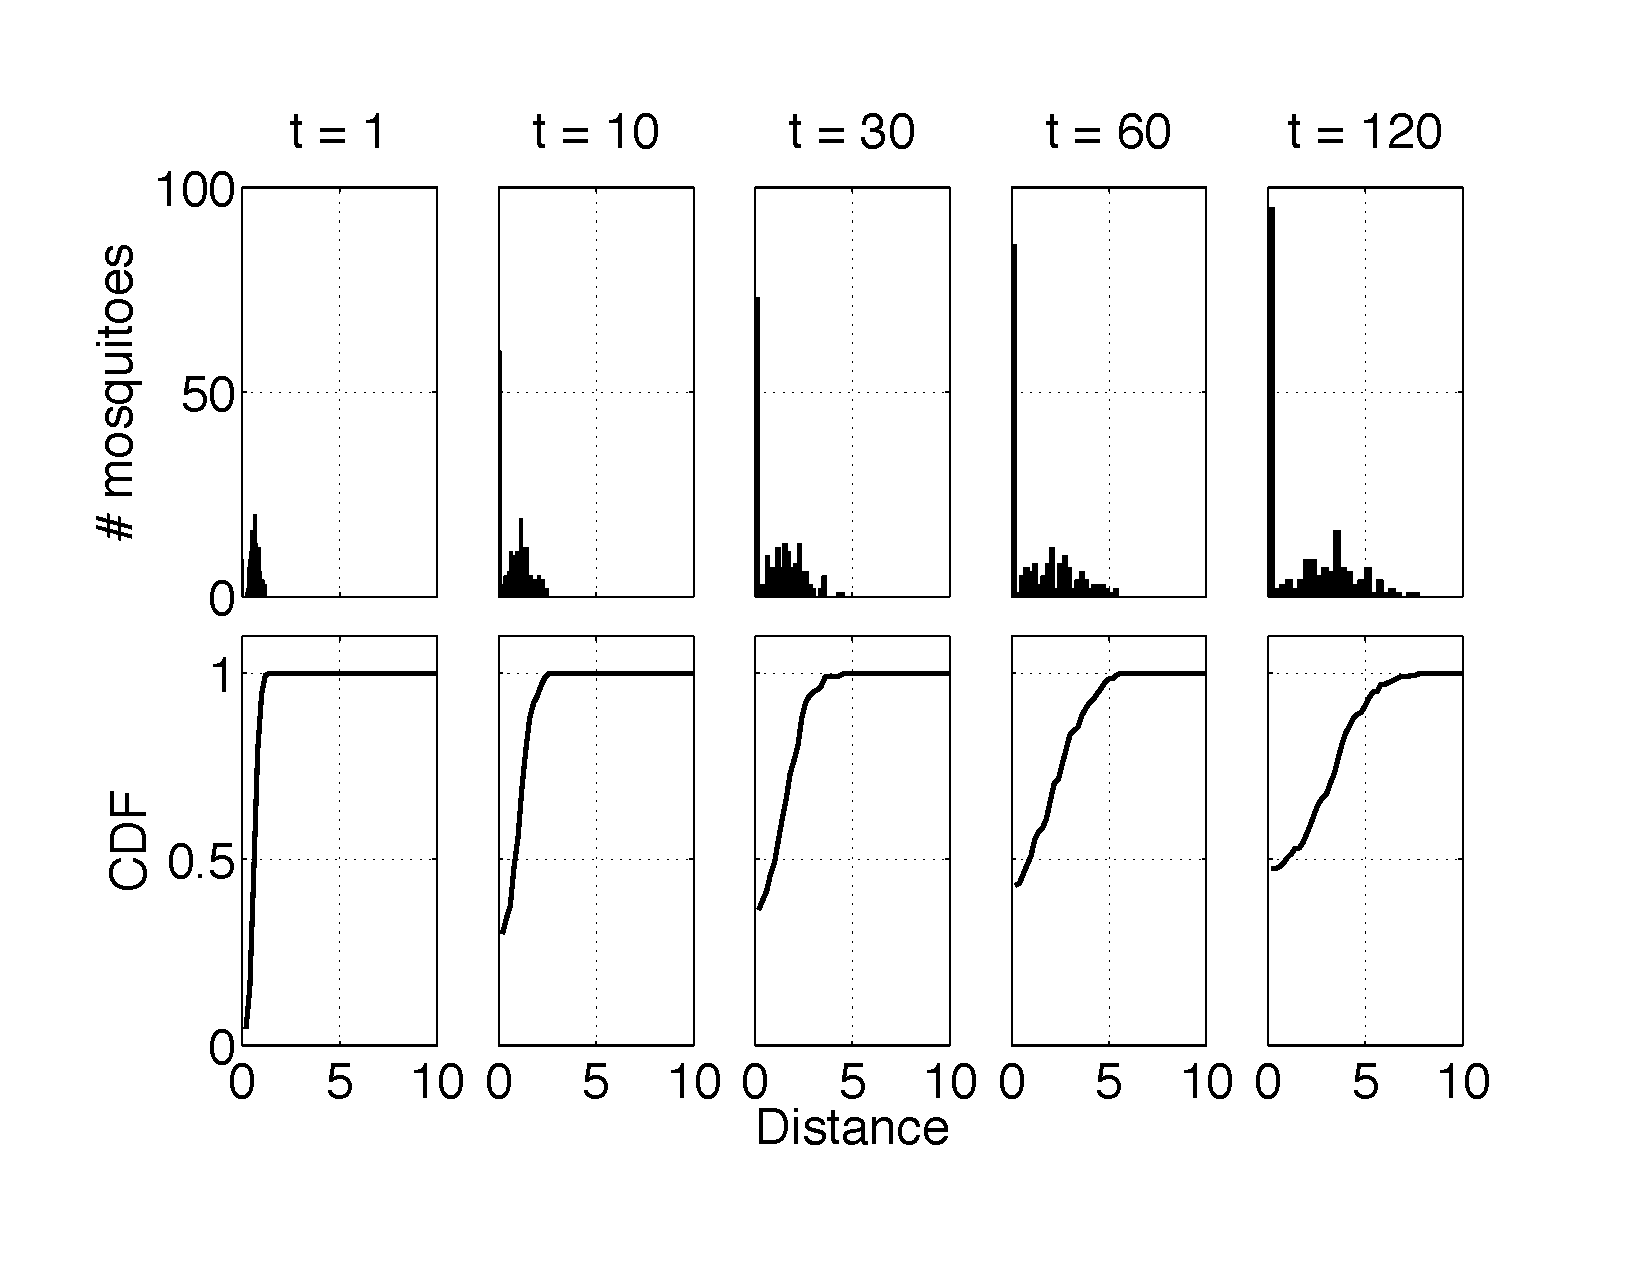
\includegraphics[width=6.8in]{figures/DiffusionFigure.pdf}
	\end{center}
	\mycaption{The distribution (upper panels) and normalized cumulative distribution (lower panels) of mosquito distances (meters) to the CO$_2$ source over time (seconds) assuming passive diffusion. Nearly half of the mosquitoes have found the source after 120 s, while the mean of the remaining mosquito distances increases with time. The CDFs will be used to calculate KS statistics within and between different rule sets.}\label{fig:diffhist}
\end{figure}

\begin{table}[hbt]
	\mycaption{Parameters for the chemotaxis homing flight rules. The $R_g$ rule set is based on knowledge of the gradient of the concentration in all directions. The $R_c$ rule set is based on the rate of change of CO$_2$ concentration sensed by the mosquito along its flight path (directional derivative).  }
	\begin{center}
		\begin{tabular}{cc}
			{\begin{tabular}{|c|c|c|c|}
				\hline
				\multicolumn{4}{|c|}{$R_g$}\\
				\hline
				\multicolumn{2}{|c|}{Direction} & \multicolumn{2}{|c|}{Speed} \\
				\multicolumn{2}{|c|}{$b=|\nabla C|/G_{sat}$} & \multicolumn{2}{|c|}{$b=C/C_{sat}$} \\
				\hline
				$\alpha_{min}$ & $\pi/2$ &    $S_{min}$ & 0.1 \\
				$\alpha_{max}$ & $\pi$ &      $S_{max}$ & 1.9 \\
				$G_0$ & 0.0833 &              $C_0$ & 0.05 \\
				$G_{sat}$ & 1.7 &             $C_{sat}$ & 0.9 \\
			    $\kappa$ & 0 &            	$\kappa$ & 0 \\
				\hline
			\end{tabular}} &
			{\begin{tabular}{|c|c|c|c|}
				\hline
				\multicolumn{4}{|c|}{$R_c$}\\
				\hline
				\multicolumn{2}{|c|}{Direction} & \multicolumn{2}{|c|}{Speed} \\
				\multicolumn{2}{|c|}{$b=\Delta C/\Delta C_{sat}$} & \multicolumn{2}{|c|}{$b=C/C_{sat}$} \\
				\hline
				$\alpha_{min}$ & $\pi/12$ &    $S_{min}$ & 0.1 \\
				$\alpha_{max}$ & $\pi$ &      $S_{max}$ & 1.9 \\
				$\Delta C_0$ & 0.0042 &              $C_0$ & 0.05 \\
				$\Delta C_{sat}$ & 0.17 &             $C_{sat}$ & 0.9 \\
			    $\kappa$ & 0 &            	$\kappa$ & 0 \\
				\hline
			\end{tabular}} 		
	\end{tabular}\label{tab:toyparams1}
	\end{center}
\end{table}
		
%%%%%%%%%%%%%%%%%%%%%%%
\subsubsection{Comparison of diffusion and Chemotaxis Rule $R_g$}
%%%%%%%%%%%%%%%%%%%%%%%
We compared diffusion with rule $R_g$ in Table~\ref{tab:toyparams1}. Under $R_g$, mosquitoes use the CO$_2$ gradient to choose direction and the concentration level to choose speed. Note from the table that far from the CO$_2$
source, where concentration is below the threshold, mosquitoes move faster under rule $R_g$
(at $S_{max}$) than the diffusion speed of 1.
We calculated the mean KS statistic over time between diffusion and $R_g$ (left panel in Fig.~\ref{fig:diffcomp}, broken line) and see that these two heuristics are significantly different as expected. Under $R_g$, many more mosquitoes find the source.
		
\begin{figure}[hbtp]
	\begin{center}
		\begin{tabular}{cc}
		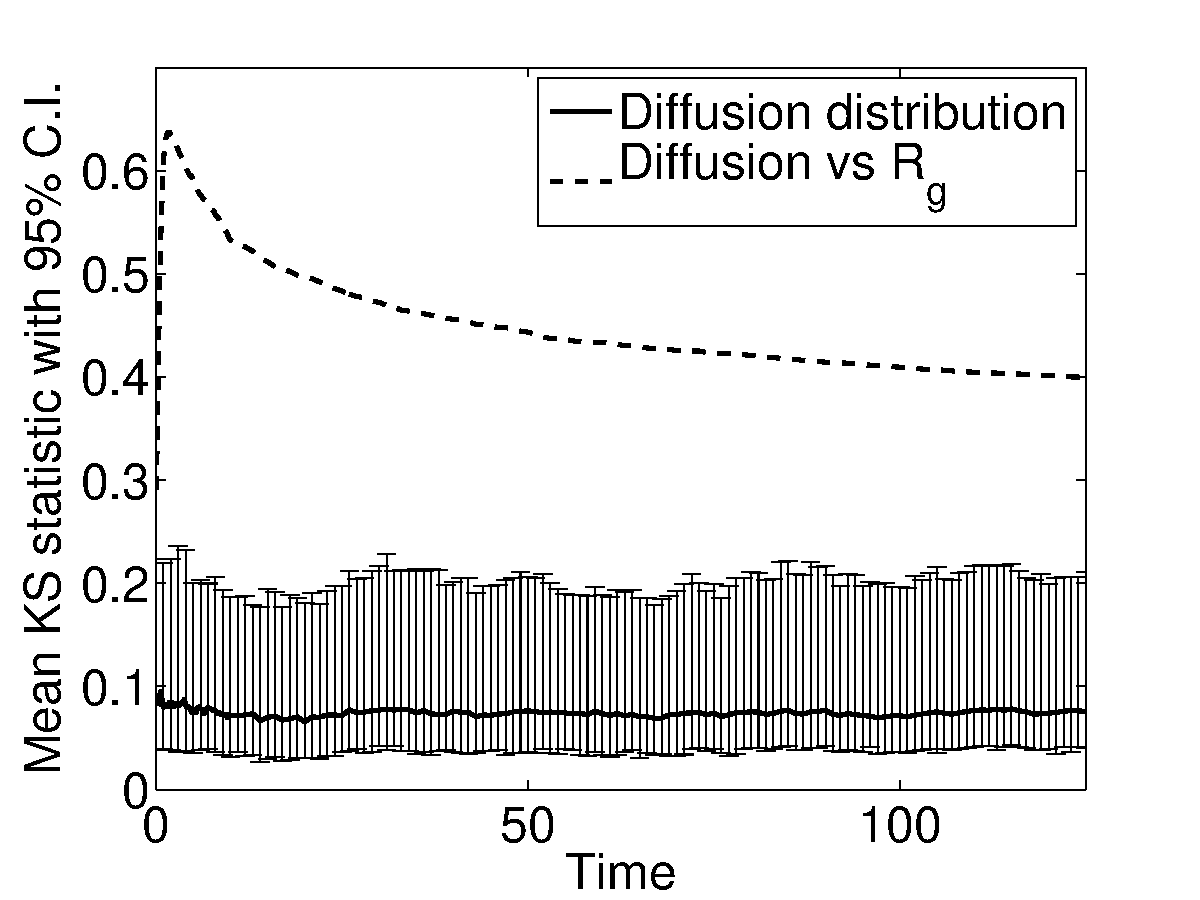
\includegraphics[width=3.25in]{figures/DiffusionvsRg.pdf} & 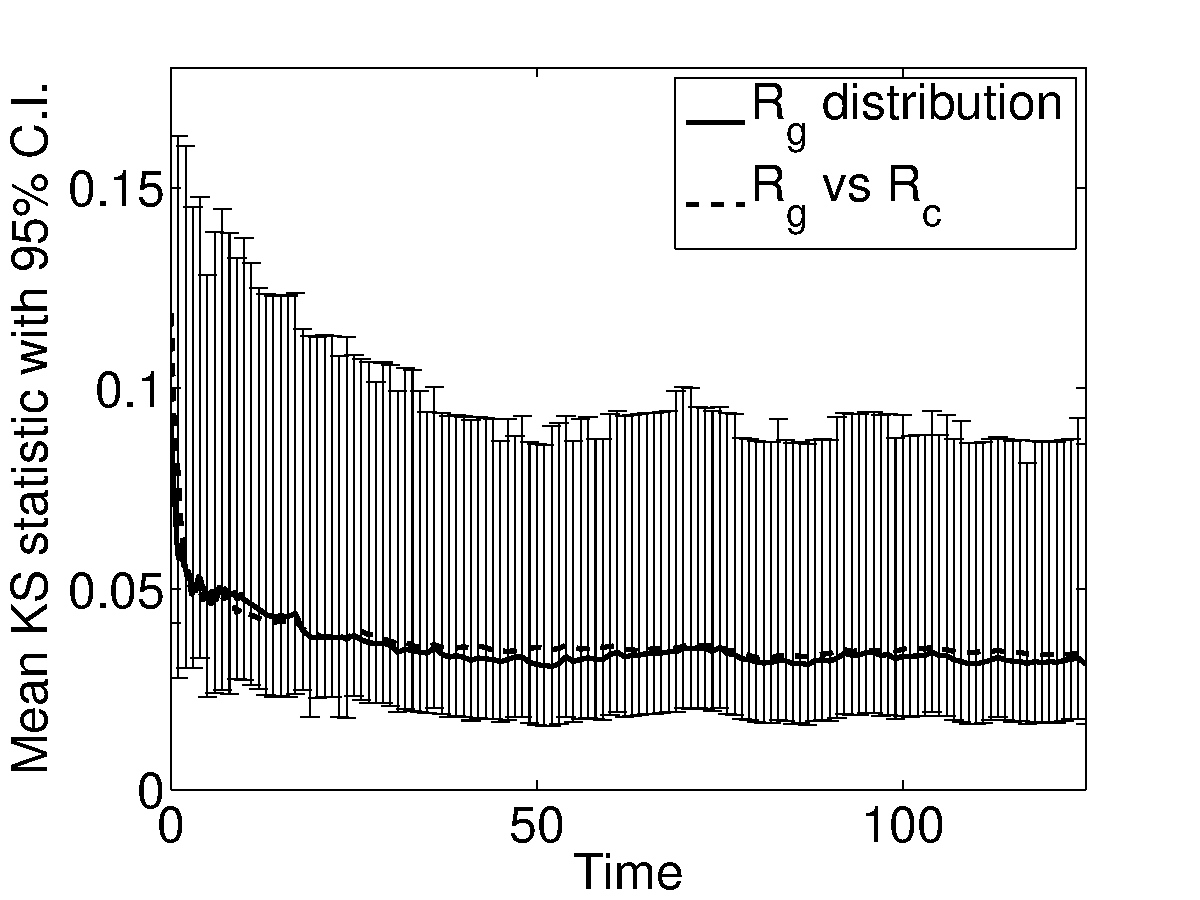
\includegraphics[width=3.25in]{figures/RgvsRc.pdf}
	\end{tabular}
	\end{center}
	\mycaption{Left panel: Diffusion vs $R_g$ with parameters from Table~\ref{tab:toyparams1}. The solid lines are the mean and 95\% confidence interval of all the pairwise KS statistics calculated within the diffusion simulations. The broken line is the mean of the KS statistics calculated between diffusion and $R_g$. Since the broken line falls so far from the diffusion confidence interval, we conclude that the two rules are highly dissimilar. Right panel: $R_g$ vs $R_c$ from Table~\ref{tab:toyparams1}. Now the solid lines are the empirical distribution for $R_g$, and the broken line is the mean of the KS statistics between $R_g$ and $R_c$. Unlike the left panel, these two rules are nearly identical.}\label{fig:diffcomp}
\end{figure}

%%%%%%%%%%%%%%%%%%%%%%%
\subsubsection{Comparison of Chemotaxis Rules $R_g$ and $R_c$}
%%%%%%%%%%%%%%%%%%%%%%%

We also compared different chemotaxis rules to each other. Figure~\ref{fig:diffcomp} (right panel) shows a comparison between rules $R_g$ and $R_c$ (see Table~\ref{tab:toyparams1}), which exhibit nearly identical behavior using the mean KS statistic. Mosquitoes using $R_c$ do not sense the CO$_2$ gradient. Instead, they compare the current concentration to the concentration at their previous location, which gives them an estimate of the gradient in their
current heading direction only (a directional derivative). In contrast, mosquitoes using $R_g$ know the gradient direction and are much more efficient in reaching the CO$_2$ source. However, if we choose the minimum window width $\alpha_{min}$ to be much lower for $R_c$ than $R_g$, then the rules are indistinguishable. For this comparison, the threshold and saturation levels used for the rules are related by $\Delta C_0 = G_0L/2$ and $\Delta C_{sat} = G_{sat}L$.


Our observations from this experiment include:
\begin{itemize}
\item
Consider rule set $R_g$ in Table~\ref{tab:toyparams1} and compare it to a new rule set $R_{gf}$  that uses
the same variable $b = |\nabla C|/G_{sat}$ to choose the flight segment direction but uses a fixed flight segment speed
$S_{max} = S_{min} = 1$.  We can find parameter values for $\alpha_{min}$, $S_{min}$ and $S_{max}$
in $R_g$ such that the mean KS statistic between $R_g$ and $R_{gf}$ is not significantly different from the KS statistic of $R_g$.
A similar conclusion is reached based on $R_c$ (instead of $R_g$) and the corresponding $R_{cf}$.

	\item
	We could not find parameter values that matched $R_c$ to $R_{gf}$ or $R_g$ to $R_{cf}$. We conclude that rules differing in both direction and speed may be difficult or impossible to match, although this may not hold under a broader parameter search.
	\item
	The match shown in Figure~\ref{fig:diffcomp} (right) between behavior rule sets $R_g$ and $R_c$ requires each rule set to have its own values of the parameters  $\alpha_{min}$, $S_{min}$, and $S_{max}$ (we fixed $\alpha_{max}=\pi$ to ensure diffusive behavior far from the source).
	 If these parameters are varied in one rule set but not varied proportionally in the other rule set, then the mean KS statistic changes sensitively. The same is true for independent variation of the thresholds and saturation levels. The match between $R_g$ and $R_c$ shows mixed sensitivity and robustness to other parameter changes:
	\begin{itemize}
		\item
		Doubling the mosquito decision flight segment time $\Delta T$ makes no substantial difference to the resulting match. Halving this flight segment time causes a noticeable but not significant mismatch at early times.
		\item
		Doubling the critical radius $r_c$ where the mosquitoes find the source does not affect the match, but halving it causes a significant mismatch at early times.
		\item
		Downward concavity ($\kappa = 1 - 1/b_0$) in Figure~\ref{MosquitoGradient} makes no substantial difference to the resulting match. Upward concavity of the angle window function ($\kappa = 200$) causes a significant mismatch at early times.
	\end{itemize}
\end{itemize}



\textbf{Final parameter choices:} Based on the model test, we choose to use the spatial gradient approach to determine direction of the mosquitoes.
Figure~\ref{fig:diffcomp} (right panel) shows that it is possible, through appropriate parameter choices, to make a rule based on the spatial gradient indistinguishable from one that uses more limited information. We may capture a wide range of potential behaviors by varying parameters, although other chemotaxis models may be easily substituted for this one. The specific chemotaxis parameters that we use for the full wind driven simulations are listed in Table~\ref{tab:finalparams}. In the remainder of this work, we set the concavity parameter $\kappa$ to be 0, corresponding to a piecewise linear response.


%%%%%%%%%%%%%%%	
\section{Sensitivity Analysis}\label{sec:SA}
%%%%%%%%%%%%%%%
Our goal is to explore the effect of host spatial distribution on the mosquito-host contact rate. To do this, we must fix a large number of parameter values governing the odor plume simulation and the mosquito behavior (see Table~\ref{tab:finalparams}). In this section, we consider a single host distribution and locally vary a collection of our model parameters independently to assess the robustness of the model with respect to our target parameter set.

We vary each of the starred parameters in Table~\ref{tab:finalparams} by $\pm$10\% while holding all other parameters constant. Figure~\ref{fig:2groups} shows the fixed arrangement of hosts for the local sensitivity analysis. Ten birds are divided into two groups, seven on the left and three on the right, with approximately the same spatial density in each group. We choose a single sequence of random velocity fields in time to superpose over the bulk flow in every realization. In order to capture the average mosquito behavior, the simulations are repeated $n$ times within each ranging behavior (upwind, downwind, and crosswind), until a mild convergence criterion is satisfied ($n \approx$ 15-20). The same sequence of random numbers are used generate mosquito behavior in each set of $n$ simulations. The differences in mosquito behavior between sets will be due solely to the parameter perturbations and not to the stochastic nature of the agents.


\begin{figure}[hbt]
	\centering
 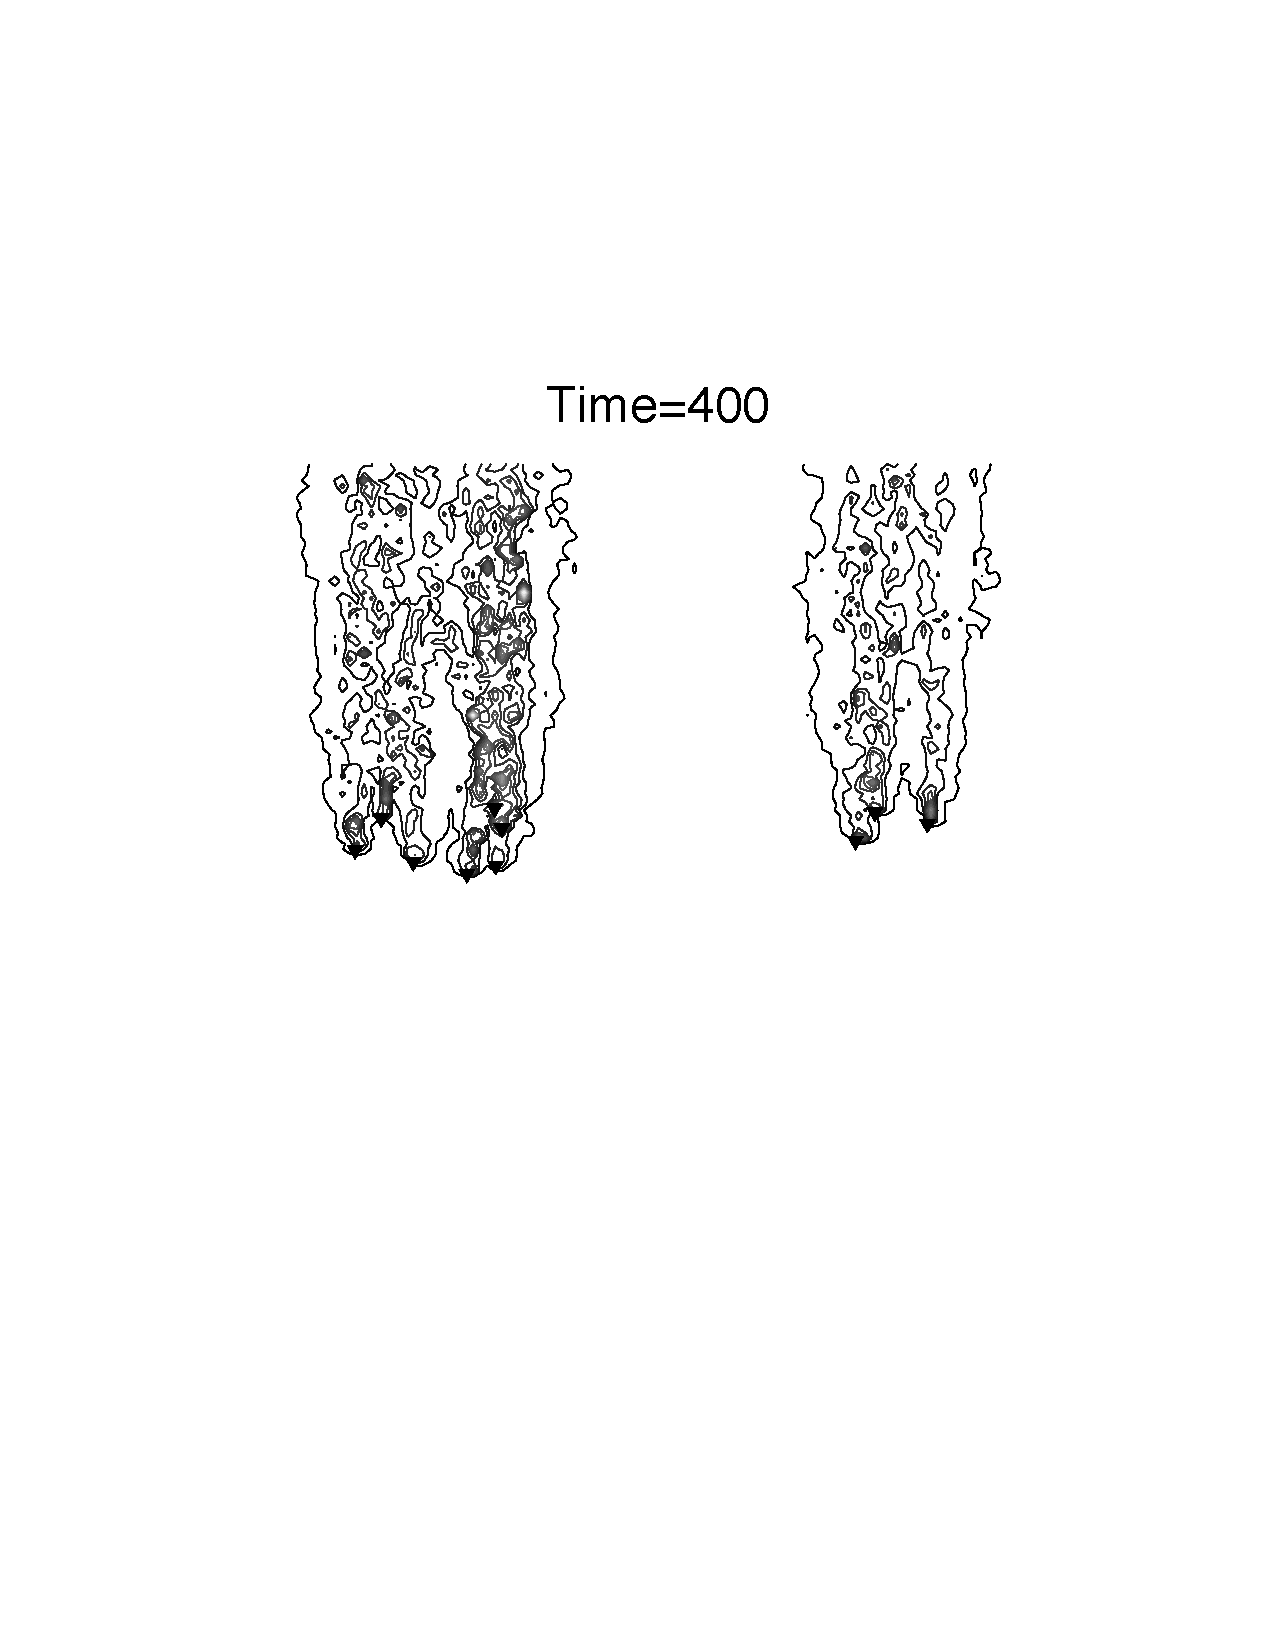
\includegraphics[width=5.0in]{figures/2groups_gray.pdf}

\mycaption{Fixed distribution of hosts for the local sensitivity analysis: seven hosts on the left and three on the right. The contours indicate nondimensional concentration and lighter colors mean higher concentration. The outermost contour is the CO$_2$ threshold. Here $L=100$, $N=128$, $\Delta t = 0.1$ for the convection-diffusion equation, and $\Delta T = 1$ for the mosquito decision making.
}
\label{fig:2groups}
\end{figure}
		


The output variables we analyzed include:
\begin{itemize}
\item the proportion of mosquitoes that find a host anywhere in the domain, $P$,
\item the proportion that find a host from the left group, $P_\ell$, and
\item the proportion that find a host the right group, $P_r = P - P_\ell$.
\end{itemize}

If we denote a generic input variable by $I$, its unperturbed value as $I^0$, and its perturbations as $I^\pm$, then our sensitivity index ($SI$) is calculated as
\begin{equation*}
	SI = \frac{P_*^+ - P_*^-}{I^+ - I^-}I^0 = \frac{P_*^+ - P_*^-}{0.2},
\end{equation*}
which is a centered difference approximation of the derivative of the output with respect to the normalized input. We estimate the variation (potential error) in this method by
\begin{equation*}
	E = \left|\frac{P_*^+ - P_*^0}{0.1} - \frac{P_*^0 - P_*^-}{0.1} \right|,
\end{equation*}
which is the difference of the one-sided derivatives.

We show the results with highest sensitivity index in Table~\ref{tab:sensitivity}. Consider the first row, which measures the sensitivity of $P$ with respect to $S_{max}$ when the mosquitoes have crosswind ranging flight behavior. The baseline value for $P$ is about 80\%. The sensitivity index is 0.1517, which means that if $S_{max}$ is varied by 10\% from its value in Table~\ref{tab:finalparams},
then approximately 1.5\% more mosquitoes will locate a host, plus or minus 0.53\% (0.1*Error/2). The highest sensitivities show changes of 1-2\% of the total mosquito population with a 10\% input change. A 1-2\% change on a scale of 35-80\% indicates that our model is locally robust to the parameter set in Table~\ref{tab:finalparams}. We do not characterize the variability with respect to stochastic effects.

\begin{table}[hbtp]
	\mycaption{Most sensitive local variation.}
	\begin{center}
		\begin{tabular}{|c|c|c|c|c|}
			\hline
			Ranging behavior & input & output (baseline value)& $SI$ & Error \\
			\hline
			\multirow{5}{*}{crosswind} & \multirow{2}{*}{$S_{max}$} & $P$ (80.2\%) & 0.1517 & 0.1064 \\
										& 						  & $P_\ell$ (44.5\%)	& 0.1050 & 0.0579 \\
										\cline{2-5}
										 & \multirow{3}{*}{$T_{cwd}$} & $P$ (80.2\%) & 0.2178 & 0.0502 \\
										& 						  & $P_\ell$	(44.5\%) & 0.1016 & 0.0280 \\
										& 						  & $P_r$ (35.6\%)	& 0.1163 & 0.0222 \\
			\hline
			\multirow{2}{*}{downwind} & $S_{max}$ & $P$ (57.6\%) & 0.1250 & 0.0536 \\
										 & $r_c$ & $P$ (57.6\%) & 0.1230 & 0.0045  \\
			\hline
		\end{tabular}
	\end{center}\label{tab:sensitivity}
\end{table}

\begin{table}[hbtp]
	\mycaption{Nondimensional parameter choices. *Starred values were locally varied in the sensitivity analysis. \comment{Is this the correct meaning of 'varied locally'  MH}  
	}
	\begin{center}
		\begin{tabular}{|c|c|c|}
			\hline
			\multicolumn{3}{|c|}{Mosquito speed in the presence of CO$_2$, $b=C/C_{sat}$} \\
			\hline
			$S_{min}$ & 0.4* & minimum mosquito flight speed\\
			$S_{max}$ & 1.5* & maximum mosquito flight speed\\
			$C_0$ & 0.01* & CO$_2$ sensing threshold\\
			$C_{sat}$ & 1 & CO$_2$ sensing saturation \\
			\hline
			\multicolumn{3}{|c|}{Mosquito CO$_2$ direction, $b=|\nabla C|/G_{sat}$} \\
			\hline
			$\alpha_{min}$ & $\pi/6$* & minimum interval width for sensing $\nabla C$\\
			$\alpha_{max}$ & $\pi$  & maximum interval width for sensing $\nabla C$\\
			$G_0$ & $C_0/10$  & gradient sensing threshold\\
			$G_{sat}$ & $(C_{sat}-C_0)/5$  & gradient sensing saturation\\
			\hline
			\multicolumn{3}{|c|}{Mosquito wind direction, $b=|\vec{V}|/V_{sat}$} \\
			 \hline
			$\alpha_{min}$ & $\pi/6$* & minimum interval width for sensing wind direction \\
			$\alpha_{max}$ & $\pi/2$ & maximum interval width for sensing wind direction \\
			$V_0$ & 0 & wind sensing threshold\\
			$V_{sat}$ & 0.5 & wind sensing saturation\\
			\hline
			\multicolumn{3}{|c|}{Wind parameters} \\
			\hline
			$\vec{U}$ & [0, 0.2] & bulk flow\\
			$\vec{U}_r$ & [X(t), Y(t)]0.15* & superposed random flow field \\
			\multirow{4}{*}{$X(t),Y(t)$} & \multirow{4}{*}{mean 0, std dev 0.5} & \\
			& & normally distributed random variables  \\
			& & changed every 20 $\Delta T$ \\
			&&\\
			\hline
			\multicolumn{3}{|c|}{Miscellaneous constants} \\
			\hline
			$\nu$ & 1.6e-4* & diffusion coefficient\\
			$\hat{J_0}$ & 0.1333* & source coefficient\\
			$r_c$ & 5* & critical radius for mosquito removal from simulation \\
			\multirow{4}{*}{$T_{cwd}$} & \multirow{4}{*}{$\Delta T$[5, 9]*} & \\
			& & duration of crosswind flight in one direction \\
			& & uniformly selected from the interval \\
			&&\\
			$N_v$ & 200 & number of mosquitoes per simulation \\
			$N_h$ & 10 & number of hosts per simulation \\
			\hline
		\end{tabular}
	\end{center}\label{tab:finalparams}
\end{table}








%%%%%%%%%%%%%%
\section{Model Simulations}
%%%%%%%%%%%%%%%
 We use the model introduced in the previous sections to address several questions pertaining to small-scale host localization.
	\begin{itemize}
		\item How do the different ranging behaviors rank in terms of effectiveness in finding a host?
		\item How does the number of contacts vary between two unequally-sized host groups?
		\item How does the number of contacts vary as the density of hosts changes in a small patch?
	\end{itemize}
In the following subsections, we describe the simulations that we performed to address these questions and we summarize our findings. In answer to the first question, we find that the most contacts occur when the mosquitoes use a crosswind strategy and are allowed sufficient time to either find a host or leave the domain permanently. In the second case, we conclude that the larger of two unequally-sized groups has a smaller per capita number of contacts. For the third question, we find that the number of contacts increases with decreasing host density within a small patch of area.
	
%%%%%%%%%%
		\subsection{Host-seeking Flight Behavior and Wind Direction}\label{sec:res:meander}
			The purpose of this section is to discover which of the mosquito ranging behaviors is more effective for different plume types. Intuitively, a crosswind flight strategy should result in a larger number of contacts than upwind or downwind behavior if the plume is straight. This is because mosquitoes adjacent to the plume are more likely to intercept it if their motion is primarily crosswind. But for a meandering plume, it is not so clear that a crosswind strategy is more effective than upwind or downwind. We simulate mosquito behavior in both straight and meandering plumes and we record the proportion of mosquitoes that find a host and the average time that it takes a mosquito to locate a host. We estimate the effectiveness of each ranging behavior using these results.
			
			
			We simulated crosswind, downwind, and upwind ranging behaviors in both straight and meandering odor plumes produced by a regular grid of nine hosts located in a single small patch in the center of the domain. The domain was 10 m on a side and the grid of hosts had a density of 1 ft$^2$ (0.09 m$^2$) within the patch area.  All parameter choices were the same as in Table~\ref{tab:finalparams} except that $\hat{J}_0 = 0.042$. The time series of random velocity fields superposed over the bulk flow was the same for all simulations. The bulk velocity field for the straight odor plume is described in Section~\ref{sec:SA}. The meandering odor plume was evolved from the velocity field
			\begin{equation*}
				\vec{U}_m = \frac{U_2}{2}\begin{bmatrix} -\sqrt{3}\cos(ay)\dfrac{x+0.1L_0}{1.1L_0} \\
				 \dfrac{\sqrt{3}}{1.1L_0 a}\sin(ay)+1\end{bmatrix},
			\end{equation*}
			where $U_2$ is the $y$-component of the bulk flow vector in the straight plume $\vec{U}$ in Table~\ref{tab:finalparams}, $L_0$ is the nondimensional length of an edge of the square domain (so that $0\leq x,y \leq L_0$), and the frequency $a$ is taken to be $40L_0/(2\pi)$ . It is easily checked that this flow is incompressible, and that the maximum magnitude of the velocity field is $U_2$ over the domain. An example of the general form of this plume with a superposed random velocity field is shown in Fig.~\ref{fig:Meander}, alongside a straight plume for comparison. The meandering plume covers more area and achieves a greater width than the straight plume. The outermost contour in both plots is $C_0$, the CO$_2$ sensing threshold of the mosquito. The other contours are equally divided between $C_0$ and the maximum concentration within each plume. The meandering plume has a maximum concentration that is approximately three times higher than that of the straight plume. Since the CO$_2$ sources are the same in both simulations, the concentration difference is due solely to the differing velocity fields.

		\begin{figure}[htp]
			\centering
			\begin{tabular}{cc}
				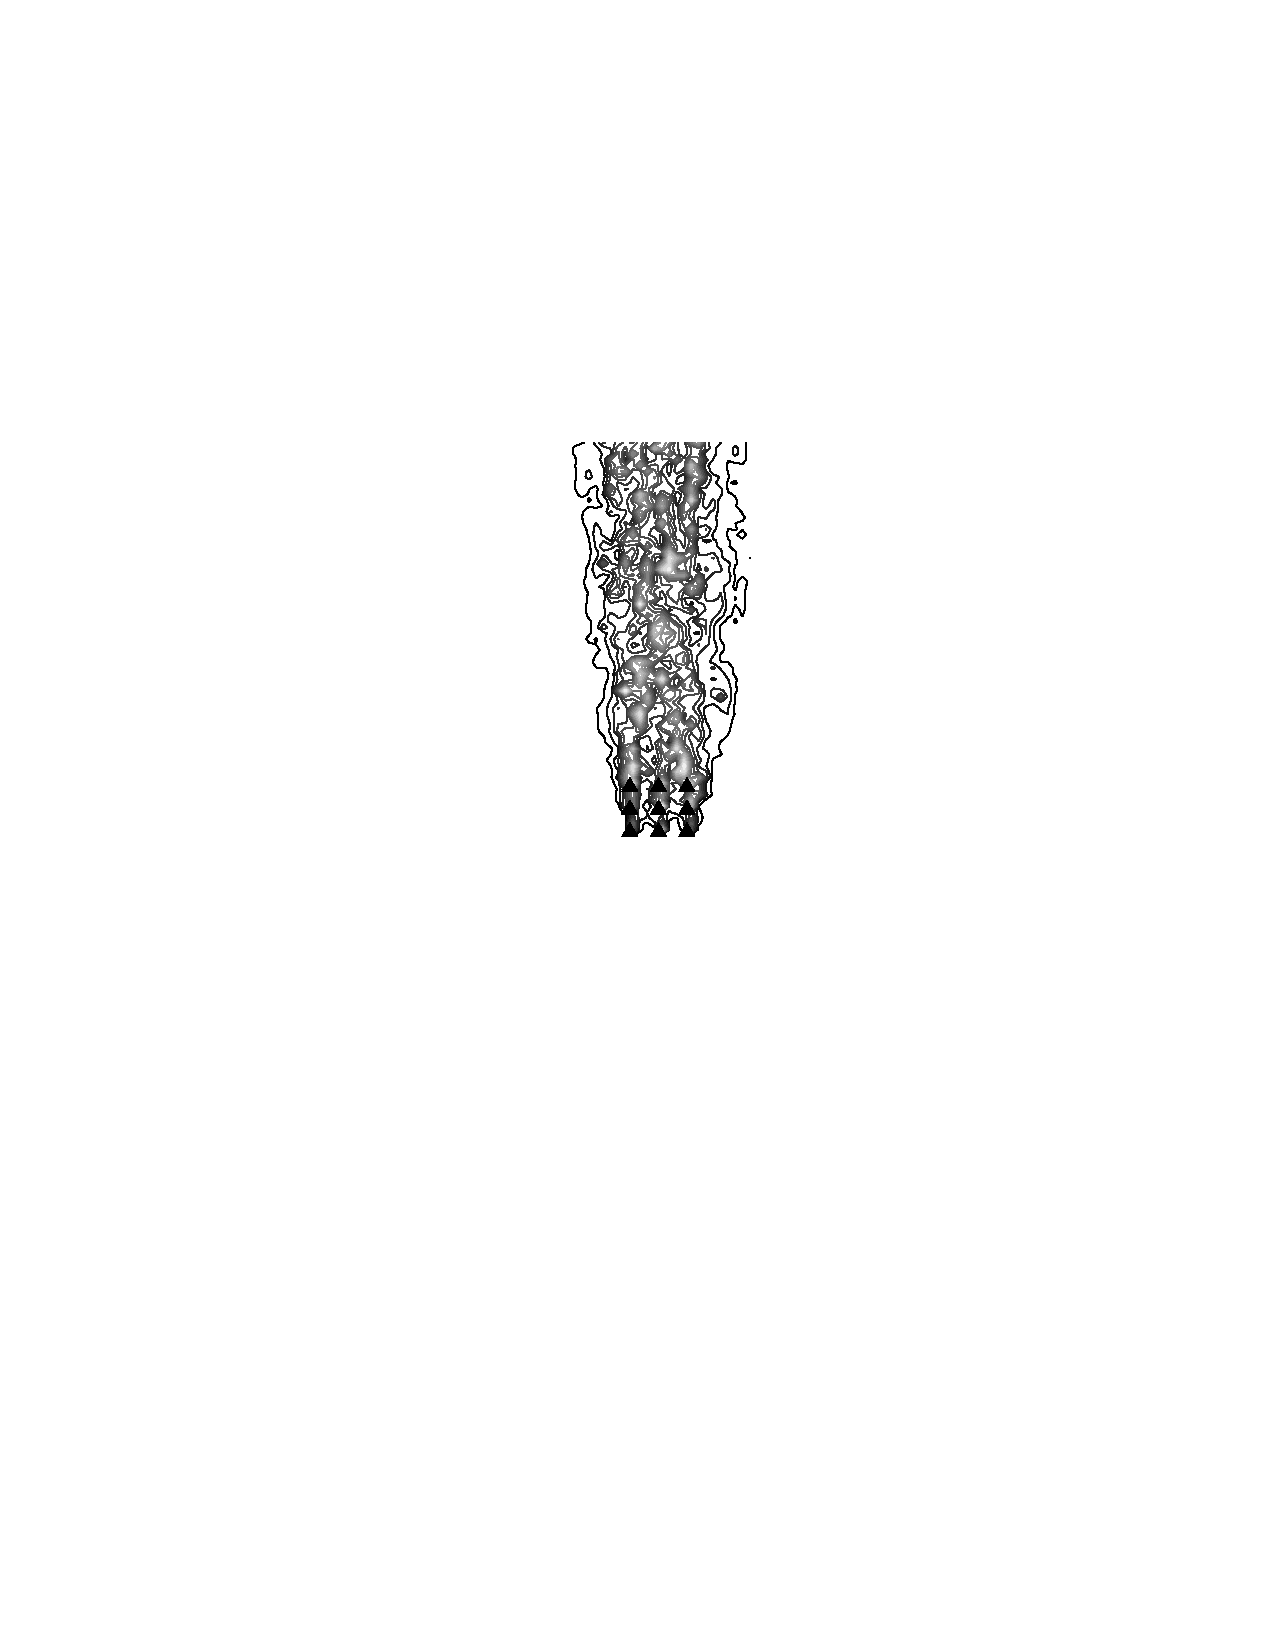
\includegraphics[width=3.3in]{figures/Results_meanderstraightpic.pdf} & 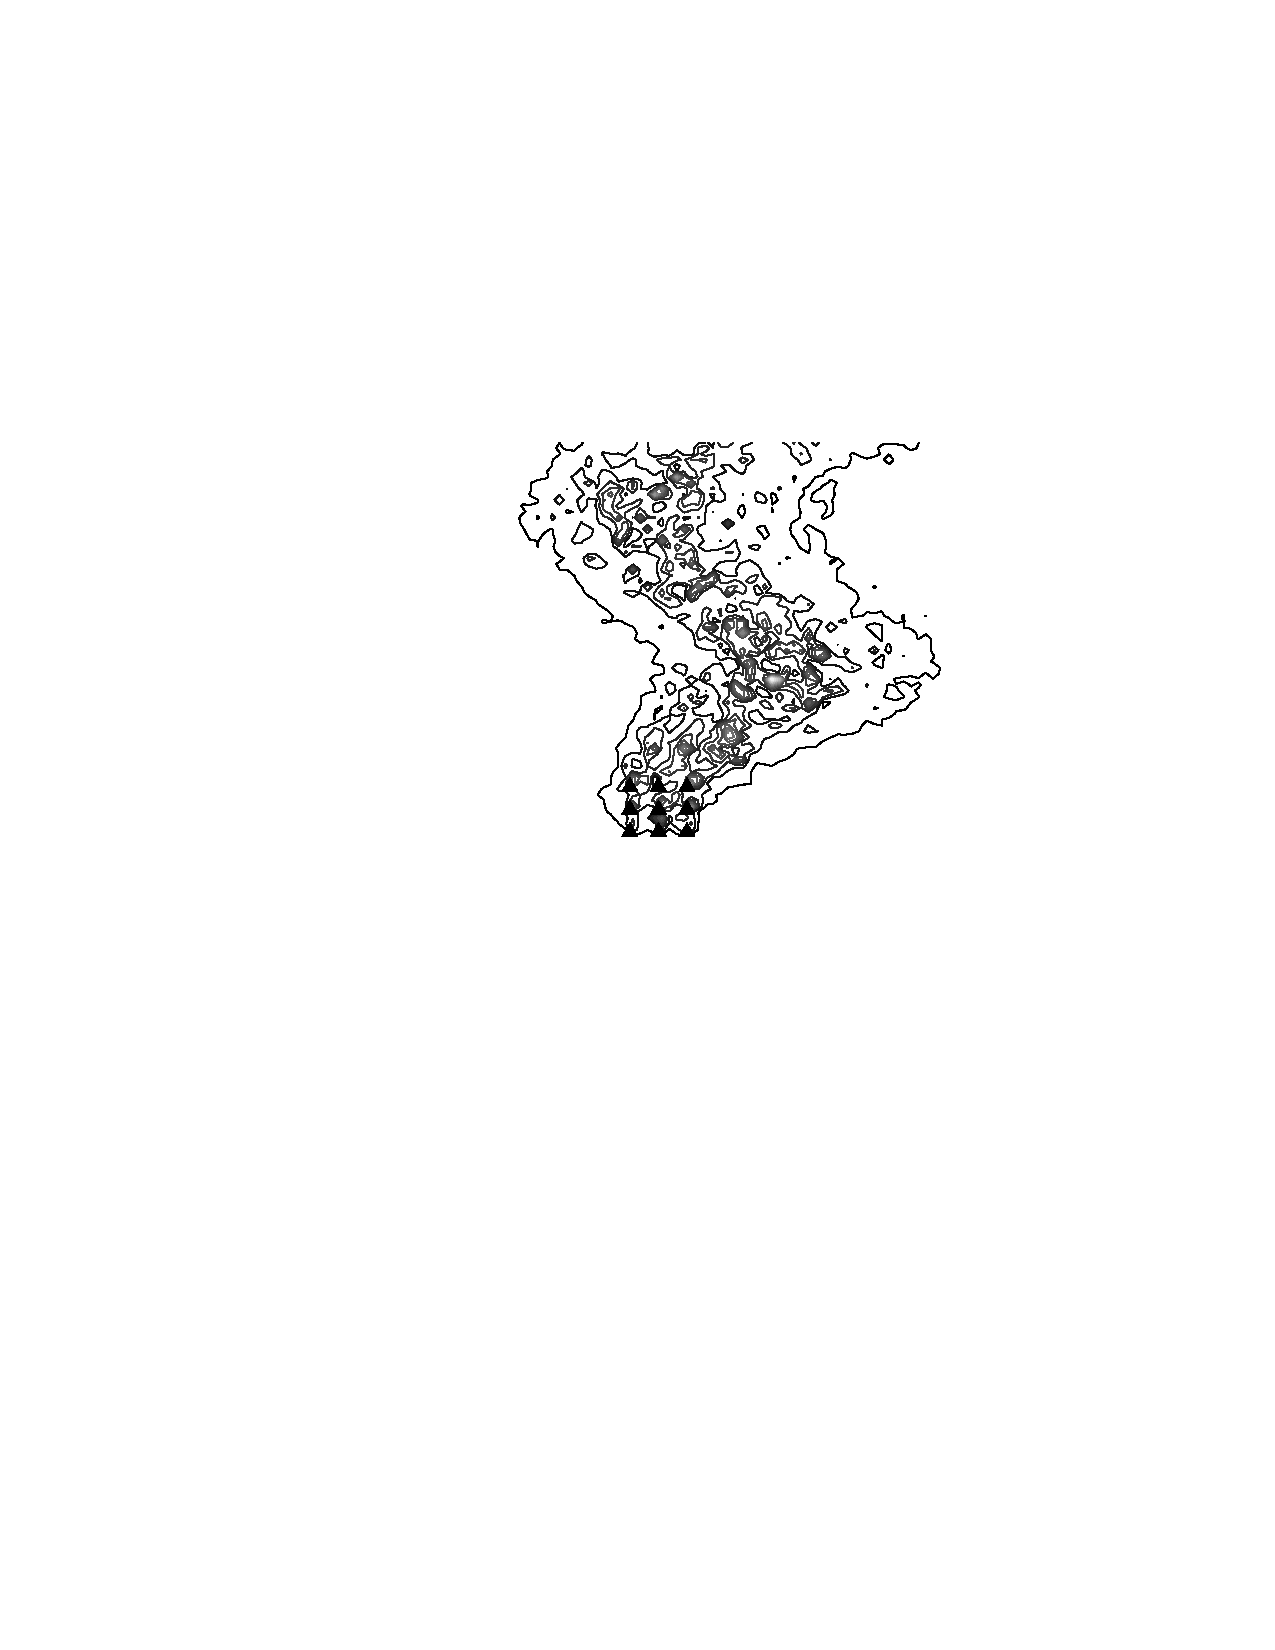
\includegraphics[width=3.25in]{figures/Results_meanderpic.pdf} \\
			\end{tabular}
			\mycaption{Examples of straight (left) and meandering (right) plumes with a superposed random velocity field (as in Table~\ref{tab:finalparams}) after the plumes have fully developed. The triangles denote host position. The contours show concentration level, with darker bars indicating lower concentration. The lowest contour is $C_0$ and is the same in both plots. The other contours are not the same in both plots because the maximum concentration is roughly three times higher in the meandering plume.}
			\label{fig:Meander}
		\end{figure}

		\begin{table}[hbtp]
			\begin{center}
				\mycaption{A comparison of ranging behaviors in straight and meandering plumes. The third and fourth columns, $P$ and std dev, are the average and standard deviation of the proportion of mosquitoes finding a host taken over 15 simulations of the same plumes with stochastic mosquito behavior. Each simulation is sufficiently long to ensure that all the mosquitoes either find a host or leave the domain. The ``average time'' column is the average time for a mosquito to find a host over all simulations, with the standard deviation taken over the \emph{means} of the simulations. The final column recalculates $P$ assuming that the simulation halts after 350 mosquito decisions.}
				\begin{tabular}{|c|c|c|c|c|c|c|}
					\hline
					Ranging behavior & plume type &$ \quad P \quad $& std dev & average time & std dev & truncated $P$\\
					\hline
					\multirow{2}{*}{upwind} & straight &20\% & 1.4\% & 111 & 5 & 20\%\\
												&  meander & 30\% & 2.0\% & 215 & 10 & 28\%\\
												\hline
					\multirow{2}{*}{downwind} & straight &23\% & 2.1\% & 47 & 6 & 23\%\\
												&  meander & 32\% & 2.7\% & 104 & 12 & 31\%\\
												\hline
					\multirow{2}{*}{crosswind} & straight &36\% & 3.3\% & 265 & 15 & 30\%\\
												&  meander & 53\% & 3.6\% & 560 & 25 & 13\%\\
					\hline
				\end{tabular}
				\label{tab:meander}
			\end{center}
		\end{table}
		
		Our results are given in Table~\ref{tab:meander}. The proportion of mosquitoes finding a host, $P$, and the average time for mosquitoes to find a host are given, along with their standard deviations. The average times are nondimensional and correspond to the number of navigational decisions a mosquito made before locating a host. The column labeled ``truncated $P$" gives the value of $P$ at time 350. We make the following observations from the table.
		\begin{itemize}
			\item The proportion of mosquitoes finding a host is \emph{larger} in the meandering plume for all ranging behaviors given sufficient time.
			\item The average time to contact a host is \emph{twice as long} in the meandering plume than the straight plume.
			\item In both plumes, a larger percentage of mosquitoes find a host using the crosswind strategy, but they take substantially longer to do so. If the mosquitoes are not time-limited in their search, then the crosswind strategy is the most effective in locating hosts.
			\item If the mosquitoes were time-limited and the simulations were stopped after 350 mosquito decisions (which is sufficient time for all upwind and downwind cases to remain unchanged), the crosswind behavior goes from being the most effective strategy in the straight plume to being the least effective strategy in the meandering plume.
		\end{itemize}
		
		From these observations we draw several conclusions.  First, a meandering plume has a higher probability of being found, but takes longer to navigate. The longer navigation in these simulations may occur because there is a longer path inside the meandering plume and also because there is a higher concentration there, which leads to slower mosquito flight. Second, if the mosquitoes are not time-limited in their search, then the crosswind strategy is the most effective in locating hosts.
			Under limited time circumstances, the crosswind behavior goes from being the \emph{most} effective strategy in the straight plume to being the \emph{least} effective strategy in the meandering plume.
			%So if there are many host patches with meandering plumes, a mosquito might find a host faster by flying downwind.
		
%%%%%%%%%%%%%%
\subsection{Distribution of Hosts}\label{sec:hostdist}
In this section we analyze the number of contacts that occur in two host groups of equal density but unequal number. One might think that the mosquitoes are drawn to each group proportionally to the number of hosts in the group. This would lead to equal per capita contacts per group. On the other hand, we might predict that the mosquitoes density is high enough so that the number of contacts is the same between both groups. Our simulations show that the results fall between these two extremes.

We performed a set of simulations in which we held the total number of hosts constant in the domain (10 birds), but split them between two groups in pairs of 9 and 1, 8 and 2, etc., down to 5 and 5 hosts per group.
All other parameters were the same as in the previous section.
%The domain was 10 m on a side and the host density was 1 ft$^2$ (0.09 m$^2$) within each group area.  All parameter choices were the same as in Table~\ref{tab:finalparams} except that $\hat{J}_0 = 0.042$.
The time series of random velocity fields superposed over the bulk flow was the same for all simulations. The two straight plumes from the host groups were well separated from each other and from the left and right domain edges. The exact positions of the hosts were allowed to vary, and the changing host position affected the shape and internal distribution of CO$_2$ over the plume.

To compare results between groups we plotted
the ratio of the mosquito-host contacts in the smaller group divided by the mosquito-host contacts in the larger group (S/L) against the ratio of the number of hosts in the smaller group over the larger group
(see Fig.~\ref{fig:2groupsres}). Each point in the error bar plot shows the mean and standard deviation over 150 simulations, corresponding to 15 simulations with stochastic mosquito behavior for each of 10 different host configurations. The diagonal line in Fig.~\ref{fig:2groupsres} denotes the case when the per capita contact rates are the same between groups. A value of 1 on the $y$-axis represents the case when the number of contacts was the same between both groups. When there are 5 hosts in both groups the number of contacts is the same, confirming that there is no left-right bias in the velocity field.

\begin{figure}[ht]
	\centering
	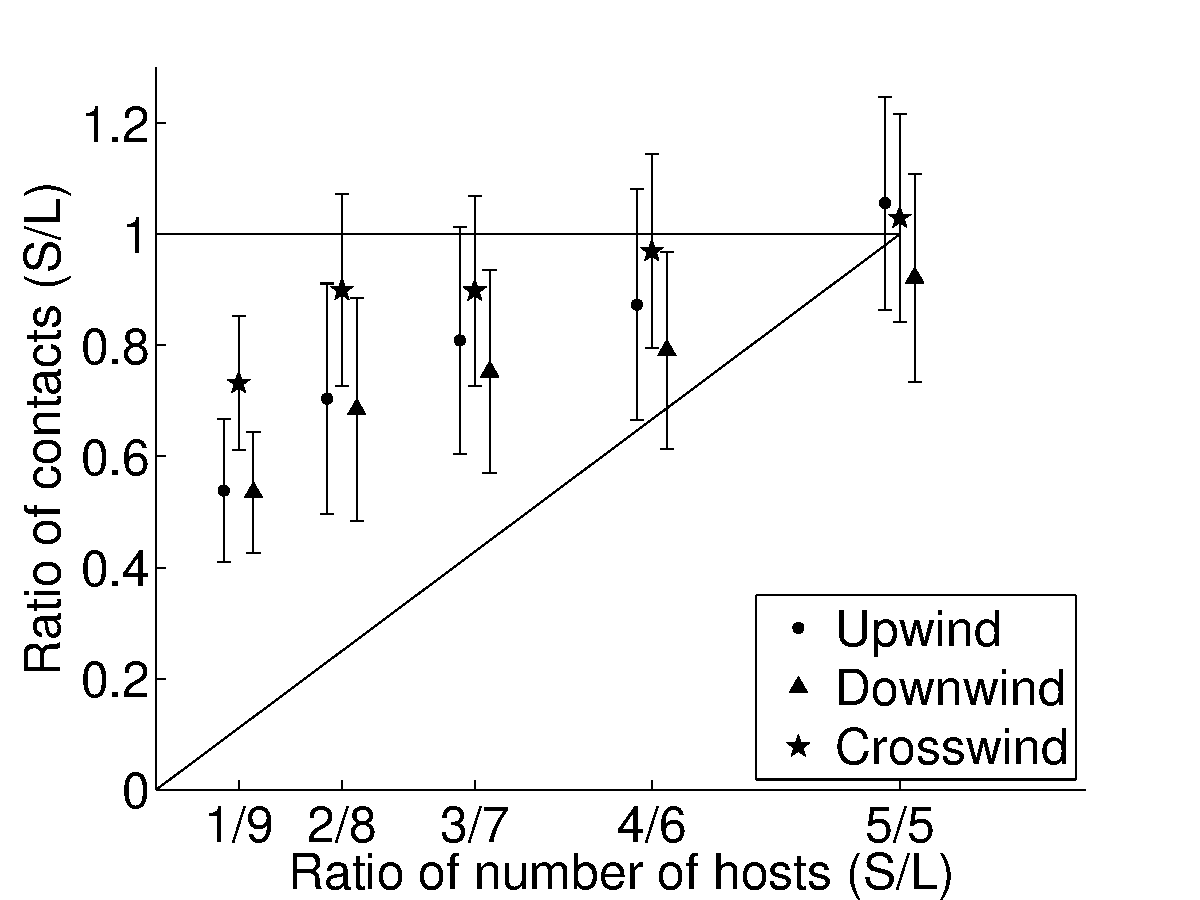
\includegraphics[width=4.25in]{figures/Results_2groups.pdf}
	\mycaption{Mean $\pm$ standard deviation of (\# contacts in the small group)/(\# contacts in the large group) plotted vs (\# hosts in the small group)/(\# hosts in the large group). The line $y=x$ shows an equal per capita contact rate between groups. Equality is not achieved until the group sizes are equal.  The data corresponding to a given ratio of hosts have been separated
	slightly in the figure for visual purposes only.}
	\label{fig:2groupsres}
\end{figure}

 When the group sizes are unequal, the per capita contact rates are higher in the small group, but the total number of contacts is higher in the large group. This occurs in the region between the lines $y=1$ and $y=x$. Of all three ranging behaviors, the crosswind strategy is closest to having equal numbers of contacts in both host groups and the downwind strategy is closest to having equal per capita contact rates. In conclusion, the number of contacts per host group is neither constant nor proportional to group size, but is intermediate between the two. Moreover, the number of contacts in each group depends on mosquito ranging behavior. These effects may only be well-captured with a small spatial scale model such as the one presented in this paper.

%	The proportion of mosquitoes finding a host, $P$, is the sum of the numbers of contacts in both the small and large groups normalized by $N_m$. In the simulations above, $P$ is approximately constant across group sizes for all ranging behaviors, varying by 1-3.5\% (data not shown). The values for $P$ in this simulation are higher than those in Section~\ref{sec:res:meander}, but the two simulations are not directly comparable due to a different number of hosts and (probably more importantly) a different set of random velocity fields.

%%%%%%%%%%%%%%%%%%%%%%%%%
\subsection{Host Density within a Patch}\label{sec:res:hostdens}
The goal of this section is to develop estimates for the proportion of mosquitoes that find a host when the hosts are restricted to a relatively small patch of space within the larger domain where mosquitoes move.  Intuitively, the size of the region where the hosts are congregated will affect the number of mosquito-host contacts for two reasons.  A larger patch of area with hosts is more likely to be found by mosquitoes in a random walk; also, the spatial arrangement of the hosts affects the shape of the odor plume they generate. In the case of constant wind velocity, we can develop estimates of the contact rate as a function of the area occupied by the hosts.

We performed a set of simulations very similar to that in Section~\ref{sec:hostdist}. In these simulations, there are 10 hosts as before, but they are in a single group in the center of the domain rather than split into two groups. Also as before, the time series of random velocity fields was held constant and the exact positions of the hosts and the mosquito trajectories were varied. We ran simulations with host density varying from 1-8 ft$^2$ per host (0.1-0.74 m$^2$), so that the area of the patch ranges from 10-80 ft$^2$ (1-7.4 m$^2$). Our domain size is approximately 1076 ft$^2$ (100 m$^2$), so that the patch size occupies less than 10\% of the domain size. For each host density, we ran 150-450 simulations to average the effects of host position and individual mosquito choices. More simulations were performed for lower host densities to achieve better coverage of the patch in which the hosts were scattered.

The proportion of mosquitoes that made contact in the group ($P$) is shown by the solid markers in both panels of Fig.~\ref{fig:Density}, with the bars corresponding to $\pm$ one standard deviation. Results for all three ranging behaviors are exhibited, and it is easily seen that crosswind ranging behavior results in the highest $P$. Upwind and downwind ranging behaviors are similar, but the upwind behavior results in a systematically lower $P$. There is a slight upward trend in $P$ with decreasing host density, corresponding to a larger host patch area. It is the shape of this curve that we seek to quantify. We derive two simple models of the curve using two different methods. The first (open markers, top panel of Fig.~\ref{fig:Density}) is based on an estimate of the plume characteristics. The second (lines, bottom panel of Fig.~\ref{fig:Density}) is a simple linear fit that depends only on the relative size of the host patch area and type of ranging behavior.
%The $x$-axis is given both in ft$^2$ per host and as the percentage of the patch area with respect to the domain area.

\begin{figure}[ht]
	\centering
	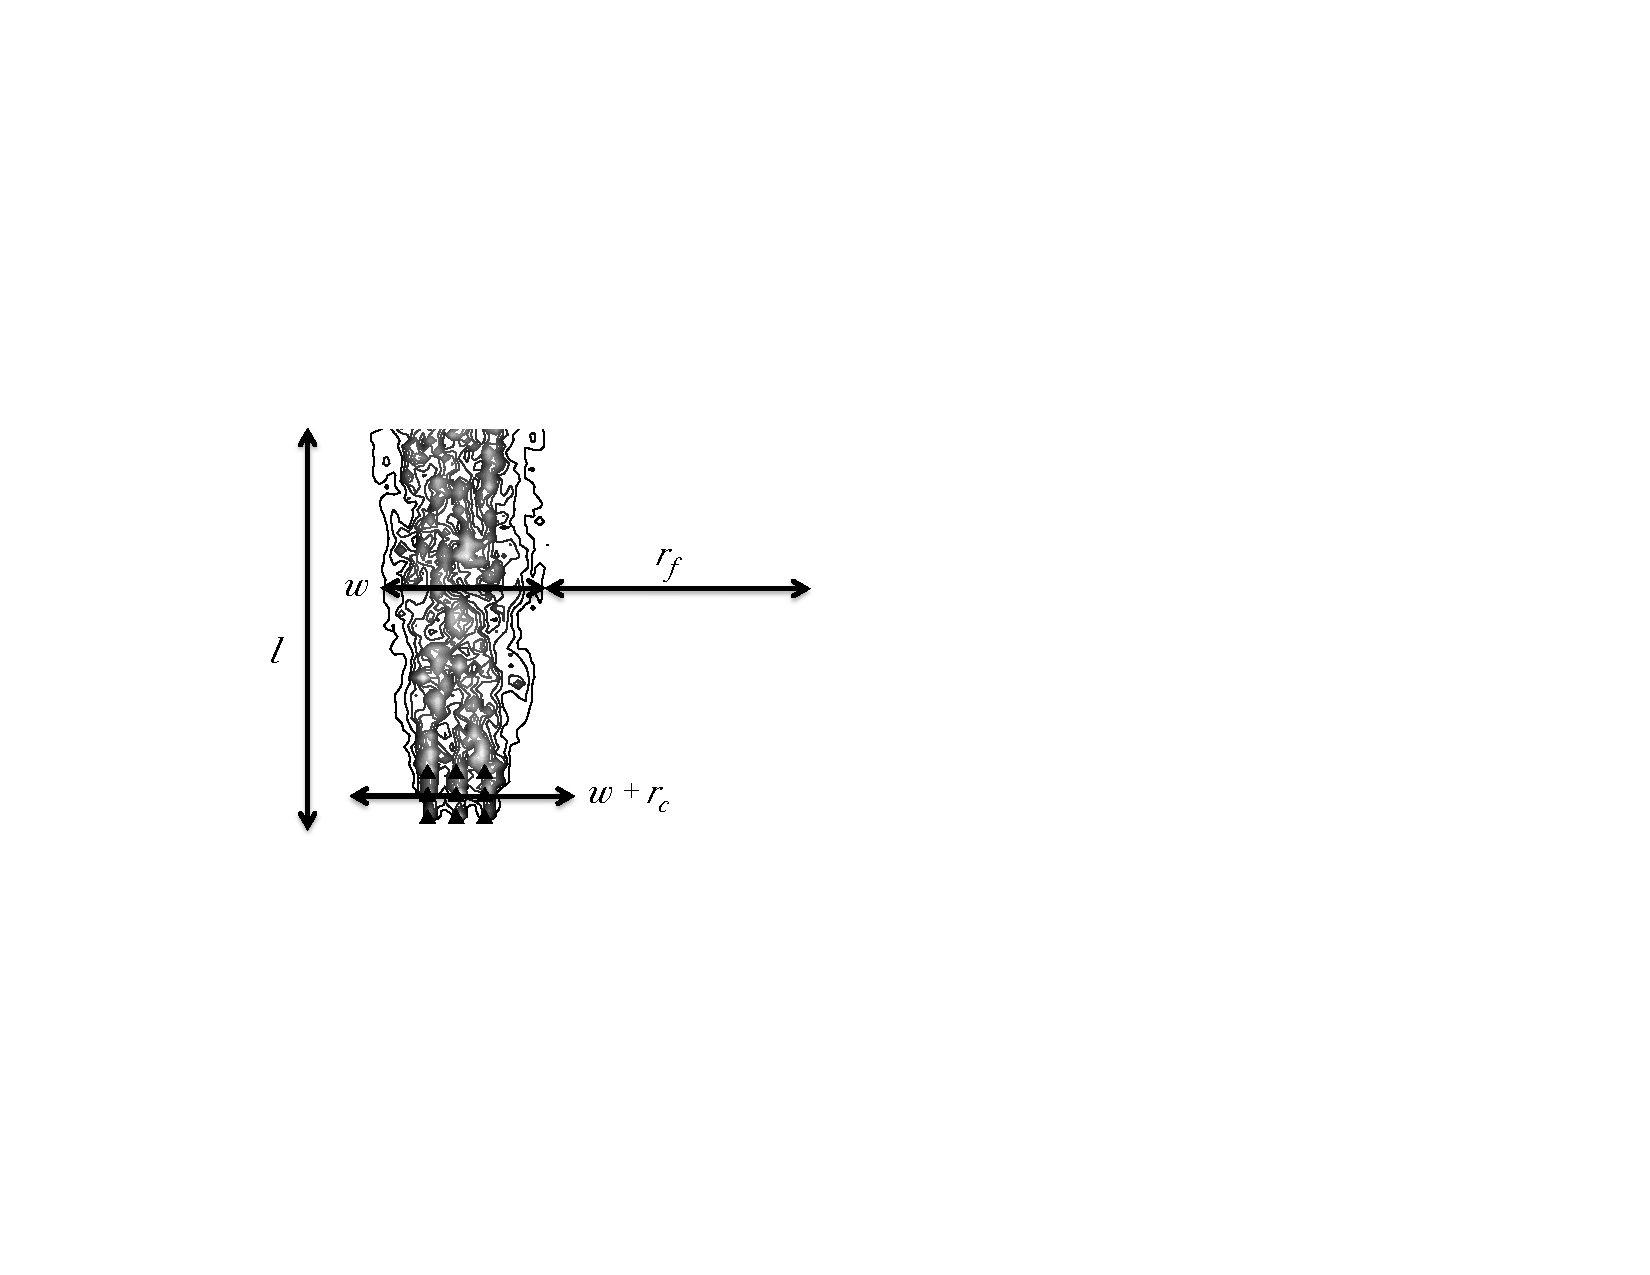
\includegraphics[width=3.5in]{figures/densitypredschematic.pdf}
\mycaption{Schematic showing the plume measurements that were estimated in order to match the results in Fig.~\ref{fig:Density}, top panel. $w$ is an estimate of maximum plume width, $r_c$ is the host critical radius (see Table~\ref{tab:finalparams}), $l$ the plume length, and $r_f$ is the average crosswind flight length for a mosquito engaging in the crosswind ranging behavior. $r_c$ and $r_f$ are constant over all runs, but $w$ and $l$ were averaged over time and over different host arrangements.}
	\label{fig:denschematic}
\end{figure}

\begin{figure}[htp]
	\centering
	\begin{tabular}{c}
	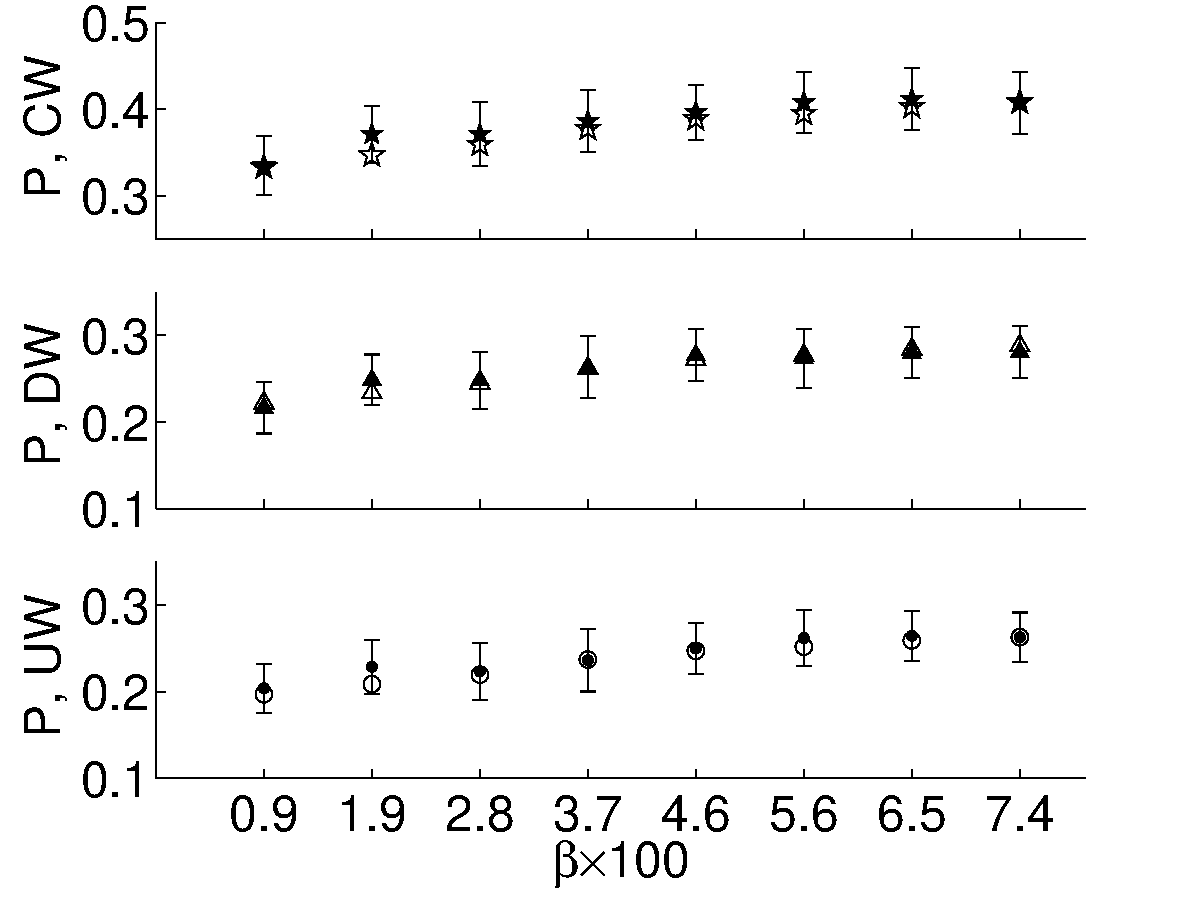
\includegraphics[width=5.4in]{figures/Results_density.pdf} \\
	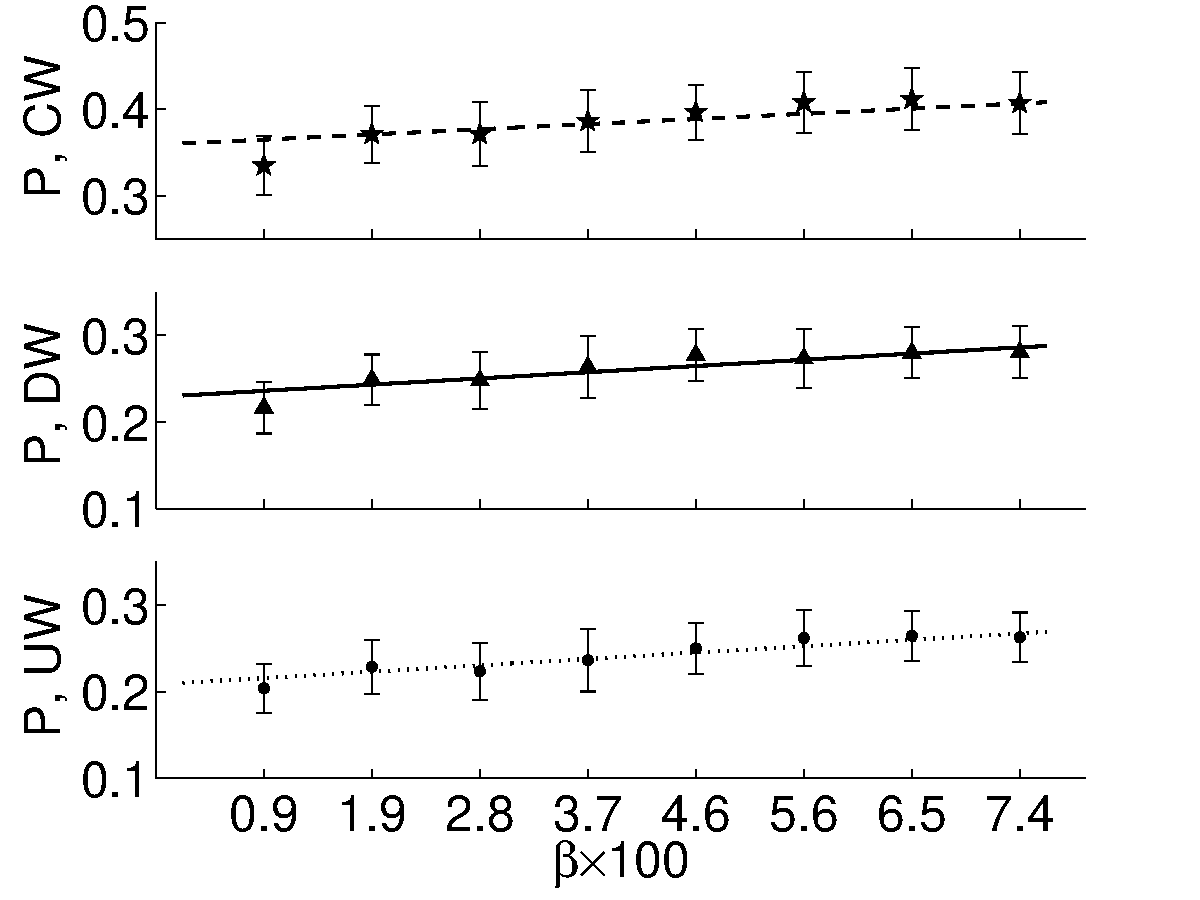
\includegraphics[width=5.4in]{figures/Results_density2.pdf}
\end{tabular}
\mycaption{Simulation results for a fixed number of hosts arranged with decreasing density given by the solid markers with $\pm$ one standard deviation (UW = upwind, DW = downwind, CW = crosswind). Top: open markers use estimates of plume width to predict contact probability. Bottom: linear fits to the data using the formula $P = c + \beta(1-c)$, where $\beta$ is the area of the host patch over the area of the whole domain. The $y$-axis is the proportion of mosquitoes finding a host. The $x$-axis is $\beta$ multiplied by 100 for ease of viewing.}
	\label{fig:Density}
\end{figure}

\textbf{Top panel, Figure~\ref{fig:Density}:} Because the plumes are straight, we can estimate their length and width over time and over different host arrangements with the same density. The edge of the plume is the contour line where $C = C_0$, the threshold CO$_2$ level. Let $w$ and $l$ be an estimate of the maximum width and the length of the plume over time for a given host density.

Consider first upwind and downwind ranging behaviors. For simplicity, we neglect any crosswind motion of the mosquitoes so that only those  that are originally lined up with the plume will find a host. In other words, the predicted proportion of mosquitoes that find a host is the width of the plume over the length of the domain. However, this would underestimate the number of mosquitoes that find a host due to the critical radius $r_c$ around each host. When a mosquito is within $r_c$ of a host, a contact is recorded and the mosquito is removed from the simulation. This effectively widens the plume, but only adjacent to host locations and not throughout the length of the plume (see the schematic in Fig.~\ref{fig:denschematic}). This means that we cannot expect to see the full benefit of widening the plume by $2r_c$, one critical radius on either side. Instead, we find that adding a fraction of $r_c$ to either side of the plume makes a good fit to the results.
The open symbols on the top panel of Fig.~\ref{fig:Density} show estimates for downwind ranging behavior (triangles) and upwind (circles) using  $P \approx (w+r_c)/L_0$ and $P \approx (w+r_c/2)/L_0$, respectively.  The crosswind estimate is discussed next.


During crosswind ranging behavior, the mosquitoes slowly drift downwind while actively flying back and forth, so mosquitoes farther away from the plume have a chance of intercepting it. To account for this, we add a term to the downwind estimate that depends on the plume length ($l$) and the average crosswind flight length ($r_f$).  Roughly speaking, a mosquito in crosswind ranging behavior may encounter the plume by either drifting downwind into the width of the plume, or by entering the region next to the plume within a distance of $r_f$. Therefore, we use the estimate $P \approx (w+r_c)/L_0 + 2(l/L_0)(r_f/L_0)$. This is a good match to our mean results (open stars, top panel of Fig.~\ref{fig:Density}).


\textbf{Bottom panel, Figure~\ref{fig:Density}:} There are two striking features of the solid markers in Fig.~\ref{fig:Density}: first, the ranging behaviors are primarily differentiated by a vertical shift, and not so much by curve shape; and second, the marker placement implies nonzero $y$-intercepts.
A patch with infinitesimally small area results in a nonzero number of mosquito-host contacts because a point source will create a finitely wide odor plume due to diffusion and random air motion. So there is a nonzero probability that mosquitoes released within a certain distance of the plume will find their way to the hosts, even as the patch area approaches zero.

We define $\beta = A_p/L_0^2$ as the ratio of the host patch area to the area of the domain and consider the linear approximation to the proportion of mosquitoes that find a host, $P  \approx c + \beta(1-c)$, where $c$ is a constant that depends on ranging behavior, number of hosts, and possibly other parameters. This linear approximation is assumed to be valid for small values of $\beta$.  We performed a least squares fit to the data to find $c$ for each ranging behavior ($c_{uw} \approx 0.21$, $c_{dw} \approx 0.23$, and $c_{cw} \approx 0.36$) and the results are the lines shown in the bottom panel of Fig.~\ref{fig:Density}.
This model is advantageous in that it depends only on the relative size of the patch and it can be directly related to a contact rate useful in standard epidemiology models. We discuss the relationship to contact rate in Section~\ref{sec:summary}.


%%%%%%%%%%%%%%%%%
\section{Summary and Discussion}\label{sec:summary}
	 %\notes{\it  {\bf Summarize your key findings in the first paragraph of the Discussion. Start by answering the question posed in introduction and relating your results to existing knowledge.}}
	 	We developed a novel hybrid agent-based/continuum model
to explore the effect of behavioral decisions and spatial heterogeneity on the encounter
rate between mosquito vectors and bird hosts. The model is flexible enough to
realistically reproduce the odor-dependent host-seeking
behavior of mosquitoes. Currently,
experimental data on the relationship between host aggregation and mosquito-host encounter rates is sparse, despite its important epidemiological implications. Our
model may offer guidance both to the planning of experimental
studies and to the interpretation of experimental data.  This work represents a first component
of  a larger model of disease transmission.


The flight direction and speed of individual mosquitoes is influenced by both the wind and odors
emitted by the hosts. The odor plumes emitted by the hosts were
tracked by a convection-diffusion equation with stochastic
variations in a directional wind to introduce sub-grid wind features. We formulated and compared
different strategies that mosquitoes might use to locate their hosts by olfaction in different wind
conditions.

%\comment{\it  {\bf Explicitly discuss (not recapitulate) the results and say what they mean. You may want to highlight, e.g. bullet, the primary results you want the reader to take away from the paper.
%At the end of the summary you may wish to discuss future directions, applications, or generalizations. Restating your key conclusions in different ways helps to reinforce your message.
%Provide the reader with your perspective and implications of what the results mean.}}

We applied our model to address three issues of potential
interest to experimental and computational epidemiologists. We
first explored the performance of different mosquito ranging
behaviors under two wind conditions. We then varied the
distribution of hosts over two groups within the computational
domain and characterized the number of contacts per group. And
lastly, we explored the effect of host patch size on the total
number of contacts made.

\paragraph{Host-seeking Flight Behavior and Wind Direction: }
We found that in general crosswind ranging flight most reliably led mosquitoes to a blood meal source, but it often took a long time. If the success of host location was discounted by the time it took (restricting success to occur after 350 or fewer navigational decisions by the mosquito) then crosswind flight was only the superior strategy in a straight odor plume. In the meandering plume, both up- and downwind searching were better than crosswind flight. This results fit very nicely with the results derived by Sabelis and Schippers~\cite{Sabelis1984} using a geometric argument.
%
\paragraph{Distribution of Hosts:} When the hosts are divided into two groups of different
size, the larger group consistently attracts more mosquitoes,
regardless of the ranging strategy, even though the difference
is less pronounced for crosswind flight than for up- or
downwind flight (Fig.~\ref{fig:2groupsres}).  Attractiveness
of a group, however, is not proportional to its relative size
(compared to the other group). Accordingly, individual hosts in
differently sized groups are subject to different contact rates.
The resulting contact heterogeneity could have important
implications for transmission dynamics. A transmission model
that does not explicitly model the resulting heterogeneity of
the contact process may not represent important characteristics
of transmission. Our model provides a tool for exploring the
effect of the distribution of hosts in 2-D space on contact
rates, given specific assumptions about the mosquitoes'
foraging strategy.
%

\paragraph{Host Density within a Patch: } Standard models of mosquito-borne transmission assume that the mosquito contact rate on one host is inversely proportional to the numbers of hosts (reviewed, e.g. by \cite{Wonham2006}). This is likely true when hosts are so abundant that a mosquito will always be able to locate one. Our simulations indicate that the chances of a mosquito to locate a host is largely determined by the width of the odor plume (Fig.~\ref{fig:Density}, top panels). The ``saturated'' situation would therefore appear to be a rare exception. However, the width of an odor plume is difficult to predict. Local wind velocity and turbulence due to landscape features will powerfully affect the shape of an odor plume. We therefore propose an approximation to the odor plume width-based model based on $\beta$ which can be viewed as a patchiness parameter (Fig.~\ref{fig:Density}, bottom panels).
This allows us to model contact rates when hosts are variably distributed over patches within a larger domain more realistically even if exact features of the relevant odor plumes are unknown.
%
%Contacts between mosquitoes and vertebrate hosts resulting from that setup are likely to be not homogenous and therefore in disagreement with the homogeneous mixing assumption of standard ordinary differential equation models. One might think of a hierarchy of models based on spatial scales in which small-scale models like the one presented here inform the parameters used in larger-scale models. We explore a possible connection in this regard. A typical term used in continuum models is the number of contacts between susceptible hosts $S_h$ and infectious vectors $I_v$ per unit time, represented by $\mathcal{N}=(S_h/N_h)(I_v/N_v)\mathcal{C}$, where $N_h$ is the total number of hosts and $\mathcal{C}$ is the total number of contacts per unit time.
This patchiness-driven contact rate model is based on the paper by
Chitnis et al.~\cite{Chitnis2006}, who propose the following contact  rate for malaria transmission
\begin{equation*}
	\mathcal{C} = \frac{\sigma_v N_v\sigma_h N_h}{\sigma_v N_v + \sigma_h N_h},
\end{equation*}
where $\sigma_v$ is the number of contacts each mosquito wants per unit time, and $\sigma_h$ is the maximum number of contacts
a host can receive per unit time. This is in the context of homogeneous mixing in a fixed area without considering
host-seeking mechanisms.

We seek to modify this expression to account for host patch area and mosquito behavior.  When there is homogeneous mixing of hosts and mosquitoes, every mosquito in a small population is expected to locate a host. This means the contact rate in the limit of a small mosquito population is $\sigma_v N_v$. But when the hosts are limited to a patch not every mosquito in a small population can be expected to make a contact, since not all of them will come into contact with the odor plume. 
% \comment{Is that backwards? I would think that small numbers of
% \emph{hosts} would lead to lower contact rates, because
% mosquitoes are less likely to successfully locate them.
% ******** MH this is what the formula does, as $N_h$ becomes small the $C$ decreases linearly with $N_h$.  I'm not sure what you are asking...  MH  ***********
% Yet I
% agree that, if there are only few mosquitoes, but they happen
% not to be where the host patches are, then overall the contact
% rate would be low. But that doesn't seem a very relevant
% scenario. IF  }
The probability of encountering an odor plume increases with
 the proportion $\beta$ of the domain in the host
patch; in the limit of a small mosquito population we assume that $\beta \sigma_v N_v$ contacts occur.
As the patch size becomes small and $\beta$ approaches
zero, the number of contacts must have a nonzero limit since
even a tiny area produces a plume that mosquitoes can follow to
a host. Based on these observations we used the modified
contact function
\begin{equation}
	\mathcal{C}_m 	= \frac{\beta\sigma_v N_v\sigma_h N_h}{\beta\sigma_v N_v + \sigma_h N_h} + P_0(1-\beta)\sigma_v N_v. \label{eqn:Cm}
\end{equation}
Note that when $\beta=1$ which represents the case of hosts
occupying the entire domain with a given spatial density, this
expression reverts to the one in the homogeneous mixing case.

In our agent-based simulations, the number of contacts per unit time can be expressed as
\[
\mathcal{C}_m = PN_v/T_s
\]
where $P$ is the proportion of mosquitoes that find a host and
$T_s$ represents the time interval between the release of
mosquitoes in the domain until they all exit the domain at the
opposite end.  We use this as our unit of time. Using the
values $\sigma_v = 1/T_s$ and $\sigma_h = N_v/T_s$ and equating
the two expressions for $\mathcal{C}_m$ leads to
\begin{equation*}
	P = \frac{\beta N_h}{\beta + N_h} + P_0(1-\beta),
\end{equation*}
where it is clear that $P_0$ represents the proportion of
mosquitoes that find a host as the patch of area containing the
hosts becomes infinitesimally small.  Note also that the
linearization of this expression for small $\beta$ is $P
\approx P_0 + \beta(1-P_0)$, which is the linear approximation
we make to the solid markers in the bottom panel of
Fig.~\ref{fig:Density}. Therefore, reasonable assumptions about the patchy distribution of hosts  in the domain allow us to devise a quantitatively reasonable estimate of the host-finding probability of mosquitoes.
%Although the fits using plume width and length in the top panel of Fig.~\ref{fig:Density} offer an alternative way of calculating $P$, it is far easier  to measure host patch area than plume shape.


%%%%%%%%%%%%%%
%\bigskip\bigskip\bigskip\bigskip
%
%The fits using plume metrics are quite good, but they involve quantities that are nearly impossible to measure in the field. It is more convenient to describe our data using patch area, number of hosts, and number of mosquitoes. A further advantage of using these particular quantities is that we may relate our findings for changing patch area to previous models of mosquito-host contact rate, and construct a modified contact rate, $\mathcal{C}_m$, that is appropriate to use when hosts are aggregated in patches. The modified contact rate can be used in compartmental models such as SIR for mosquito-borne diseases. For example, to model the number of susceptible hosts moving into the infected class, one would use $dI_h/dt = (S_h/N_h)(I_v/N_v)p_b p_t\mathcal{C}_m + $ other terms, where $S_h/N_h$ is the proportion of susceptible hosts, $I_v/N_v$ is proportion of infectious mosquitoes, $p_b$ is the probability of a successful bite given a contact, and $p_t$ is the probability of successful transmission given a bite.
%
%We will find a reasonable form for $\mathcal{C}_m$ by imposing three limits. In the limit that the host patch area approaches the domain area and that the mosquitoes are uniformly distributed over the domain, we would like to recover a known model of vector-host contact rate. We use the model of Chitnis et al.~\cite{Chitnis2006} as this limit
%\begin{equation*}
%	\mathcal{C} = \frac{\sigma_v N_v\sigma_h N_h}{\sigma_v N_v + \sigma_h N_h},
%\end{equation*}
%where $N_v$ and $N_h$ are the numbers of vectors and hosts respectively, $\sigma_v$ is the number of contacts each mosquito wants per unit time, and $\sigma_h$ is the maximum number of contacts a host can receive per unit time. In symbols, we require $\lim_{\beta \to 1} \mathcal{C}_m = \mathcal{C}$, where $\beta$ is the ratio of host patch area to domain area. Secondly, we require that $ \mathcal{C}_m \leq \sigma_v N_v$ in the limit of small mosquito populations. This means that the total number of contacts cannot exceed the total number desired by the mosquito population. Note that the first two limits combined imply that $\mathcal{C}_m$ acts like $\sigma_v N_v$ for small $N_v$ when $\beta = 1$. That is, every mosquito is expected to make a contact with a host when the mosquito population is small and uniformly mixed with a host population. Lastly, we enforce $\lim_{\beta \to 0} \mathcal{C}_m = c \sigma_v N_v$, where $c$ is the appropriate $y$-intercept for the mosquito ranging behavior (see Sec.~\ref{sec:res:hostdens}).
%
%The last limit requires some explanation. The quantity $\mathcal{C}_m$ is related to the proportion of mosquitoes finding a host, $P$, by the relationship $\mathcal{C}_m = PN_v/T_s$, where $T_s$ is the length of the simulation in time. This is simply the total number of contacts made, $PN_v$, divided by the total time it took to make the contacts, $T_s$. In the context of our simulations, every mosquito wants one bite so we take the desired biting rate to be $\sigma_v = 1/T_s$. Then $\mathcal{C}_m = P\sigma_vN_v$, which means the last limit above is equivalent to $\lim_{\beta \to 0} P = c$, which is the empirical limit that we see the bottom panel of Fig.~\ref{fig:Density} (recall that $c$ depends on the ranging behavior). Note that $c \leq 1$ by the definition of $P$.
%
%One expression that fulfills all of these limits is
%\begin{equation}
%	\mathcal{C}_m 	= \frac{\beta\sigma_v N_v\sigma_h N_h}{\beta\sigma_v N_v + \sigma_h N_h} + c(1-\beta)\sigma_v N_v. \label{eqn:Cm}
%\end{equation}
%The limits for $\beta$ are easily seen. As the mosquito population becomes small, $\mathcal{C}_m \approx (\beta(1-c) + c)\sigma_v N_v$. Since $0 \leq \beta \leq 1$ implies that $c \leq \beta(1-c) + c \leq 1$, our second requirement is satisfied.
%
%We now show the connection between the linear fits $P  \approx c + \beta(1-c)$ in the bottom panel of Fig.~\ref{fig:Density} and the modified contact rate in Eq.~\eqref{eqn:Cm}. We do not model an upper bound for the number of bites a host can receive, so we take $\sigma_h = N_v/T_s$. This states that a host may receive all possible bites over the course of a simulation. Using this substitution and those for $\sigma_v$ and $\mathcal{C}_m$, we have
%\begin{equation*}
%	P = \frac{\beta N_h}{\beta + N_h} + c(1-\beta).
%\end{equation*}
%For small $\beta$, this equation reduces to $P  \approx c + \beta(1-c)$, which we use to find the appropriate value of $c$ for each ranging behavior from the solid markers in Fig.~\ref{fig:Density}.
%



 %\comment{\it  {\bf  Put your new results in the context of the overall status of the field.  Explain what is new without exaggerating, and be sure to not just repeat your results. It is fine to reference previous tables and figures. Do not speculate or over discuss results and be sure to discuss weaknesses and discrepancies.  }}
Our model provides insight into the effect of host aggregation on how mosquitoes distribute their blood feeding among these hosts, given the assumption we make on odor plume dispersal and mosquito behavior. Very little experimental data exists on these processes. Because of the central role blood feeding plays in the transmission dynamics of mosquito-borne disease our model therefore may offer important insight into the mechanics of transmission on a small spatial scale.

In the future, our mosquito behavior model could be extended to longer time and larger spatial scales. Disease transmission via mosquito bite, host movement, infection, and demographic processes in both vertebrate hosts and mosquitoes and the dependence of these processes on biotic and abiotic factors could be integrated with the existing model for explicit small scale modeling of disease spread. There is virtually no limit to further levels of complexity that could be added to this (gusting wind, moving hosts, variable breathing rate, compound odors etc). The challenge will be to identify the components that most strongly affect the behavior of the model system and the underlying reality on which it is based.
 %
%
A simulation model of mosquito-borne transmission that integrates our mosquito-host contact model will then allow us to evaluate spatial effects  at a ``small'' scale (e.g. as measured in mosquito flight range) on transmission dynamics of mosquito-borne transmission.
%
\section*{Acknowledgement}
We would like to thank to Angela ...  who contributed to the development of this model at an earlier stage. This project was funded by a Tulane Research Enhancement Phase 2 Grant.
%
\bibliographystyle{plain}	
\newpage  \bibliography{biblio}
%\input{biblio.bbl}

\end{document}
